% changelog: "0.9.0, 2024-05-31, Davide Donanzan, Tracciamento test sistema"

\documentclass[8pt]{article}
\usepackage[italian]{babel}
\usepackage[utf8]{inputenc}
\usepackage[letterpaper, left=1in, right=1in, bottom=0.75in, top=0.75in]{geometry}
\usepackage{amsmath}
\usepackage{subfiles}
\usepackage{lipsum}
\usepackage{csquotes}
\usepackage{amsfonts}
\usepackage[sfdefault]{plex-sans}
\usepackage{float}
\usepackage{pifont}
\usepackage{mathabx}
\usepackage[euler]{textgreek}
\usepackage{makecell}
\usepackage{tikz}
\usepackage{wrapfig}
\usepackage{siunitx}
\usepackage{amssymb} 
\usepackage{tabularx}
\usepackage{adjustbox}
\usepackage[document]{ragged2e}
\usepackage{floatflt}
\usepackage[hidelinks]{hyperref}
\usepackage{graphicx}
\usepackage{hyperref}
\setcounter{tocdepth}{4}
\usepackage{caption}
\usepackage{multicol}
\usepackage{tikz}
\setlength\parindent{0pt}
\captionsetup{font=footnotesize}
\usepackage{fancyhdr} 
\usepackage{graphicx}
\usepackage{capt-of}% 
\usepackage{booktabs}
\usepackage{varwidth}
\usepackage{datetime2}
\usepackage{xcolor}
\usepackage{longtable}
\usepackage{array}
\usepackage{ragged2e}
\usepackage{colortbl}
\usepackage{verbatim}
\usepackage{enumitem}

\newcommand{\customtitle}{PIANO DI QUALIFICA}% o ESTERNO

% -- STILE COLONNA CENTRATA PER TABELLE -- %
\newcolumntype{M}[1]{>{\centering\arraybackslash}m{#1}}

% -- STILE INTESTAZIONE -- %
\fancypagestyle{mystyle}{
	\fancyhf{} 
	\fancyhead[R]{
\includegraphics[height=1cm]{../../template/images/logos/NaN1fy_logo.png}} 
	\fancyhead[L]{\leftmark} 
	\renewcommand{\headrulewidth}{1pt} 
	\fancyhead[L]{\customtitle} 
	\renewcommand{\headsep}{1.3cm} 
	\fancyfoot[C]{\thepage} 
}

% -- PER LA FIRMA -- %
\newcommand{\signatureline}[1]{%
	 \par\vspace{0.5cm}
	\noindent\makebox[\linewidth][r]{\rule{0.2\textwidth}{0.5pt}\hspace{3cm}\makebox[0pt][r]{\vspace{3pt}\footnotesize #1}}%
}

% -- PER IL GLOSSARIO -- %
\newcommand{\glossterm}[1]{#1\textsuperscript{G}} % inserisci \glossterm{termine}

% -- per abilitare 4x sottosezioni es 2.1.1.1
\setcounter{secnumdepth}{4}
\newcommand{\subsubsubsection}[1]{\paragraph{#1}\mbox{}\\\\}

\begin{document}
\definecolor{myblue}{RGB}{23,103,162}
\begin{titlepage}
	\begin{tikzpicture}[remember picture, overlay]
		\node[anchor=south east, opacity=0.2, yshift = -4cm, xshift= 2em] at (current page.south east) {
\includegraphics[width=0.7\textwidth, trim=0cm 0cm 5cm 0cm, clip]{../../template/images/logos/Universita_Padova_transparent.png}}; 
		\node[anchor=north west, opacity=1, yshift = 4.2cm, xshift= 1.4cm, scale=1.6] at (current page.south west) {
\includegraphics[width=4cm]{../../template/images/logos/NaN1fy_logo.png}};
	\end{tikzpicture}
	
	\begin{minipage}[t]{0.47\textwidth}
		{\large{\textsc{Destinatari}}
			\vspace{3mm}
			\\ \large{\textsc{Prof. Tullio Vardanega}}
			\\ \large{\textsc{Prof. Riccardo Cardin}}
		}
	\end{minipage}
	\hfill
	\begin{minipage}[t]{0.47\textwidth}\raggedleft
		{\large{\textsc{Redattori}}
			\vspace{3mm}
			{\\\large{\textsc{Guglielmo Barison}\\}} % massimo due 
			{\large{\textsc{Davide Donanzan}}}
			
			
		}
		\vspace{8mm}
		
		{\large{\textsc{Verificatori}}
			\vspace{3mm}
			{\\\large{\textsc{XXXX XXXX}\\}} 
			{\large{\textsc{XXXX XXXX}}}
			
		}
		\vspace{4mm}\vspace{4mm}
	\end{minipage}
	\vspace{4cm}
	\begin{center}
		\begin{flushright}
			{\fontsize{30pt}{52pt}\selectfont \textbf{Piano Di Qualifica}} % o ESTERNO
		\end{flushright}
		\vspace{3cm}
	\end{center}
	\vspace{10 cm}
	{\small \textsc{\href{mailto: nan1fyteam.unipd@gmail.com}{nan1fyteam.unipd@gmail.com}}}
\end{titlepage}
\pagestyle{mystyle}
\section*{Registro delle Modifiche}
\begin{table}[ht!]	
	\centering
	\begin{tabular}{p{1.2cm} p{2cm} p{6cm} p{3cm} p{2cm}}
		\toprule
		\textbf{Versione}& \textbf{Data} & \textbf{Descrizione} & \textbf{Autore} & \textbf{Ruolo} \\
		\midrule
        0.9.0 & 2024-05-31 & Stesura0 sezione ``Tracciamento test di sistema". & Davide Donanzan & Redattore \\\\
        0.8.0 & 2024-05-30 & Completamento della sezione ``Cruscotto delle qualità". & Davide Donanzan & Redattore \\\\
        0.7.0 & 2024-05-29 & Aggiunta di ulteriori test di unità, integrazione, sistema e accettazione. & Davide Donanzan & Redattore \\\\
        0.6.0 & 2024-05-28 & Stesura sezione ``Liste di controllo". & Guglielmo Barison & Redattore \\\\
        0.5.0 & 2024-05-24 & Stesura sezione ``Cruscotto della qualità". & Davide Donanzan & Redattore \\\\
        0.4.0 & 2024-05-21 & Stesura sezione ``Test di accettazione". & Guglielmo Barison & Redattore \\\\
        0.3.1 & 2024-05-15 & Modifiche minori alla struttura di ``Test di Unità". & Davide Donanzan & Redattore \\\\
		0.3.0 & 2024-05-14 & Inizio stesura ``Test di Unità" e ``Test di Integrazione". & Davide Donanzan & Redattore \\\\
		0.2.0 & 2024-04-28 & Inizio stesura ``Strategie di testing". & Guglielmo Barison & Redattore \\\\
		0.1.0 & 2024-04-18 & Stesura ``Obiettivi di qualità". & Guglielmo Barison & Redattore \\\\
		0.0.0 & 2024-04-09 & Struttura di base ed introduzione.  & Guglielmo Barison & Redattore \\
		\bottomrule
		% Ruolo Redattore o Verificatore
	\end{tabular}
	\caption*{Tabella: Registro delle modifiche.}
	\label{table:Registro delle modifiche}
\end{table}
\newpage
\tableofcontents
\newpage
\listoffigures
\newpage
\listoftables
\newpage
\justifying
\section{Introduzione}
\subsection{Scopo del documento}
Questo documento offre una panoramica dettagliata delle strategie di verifica e validazione adottate per assicurare la \glossterm{qualità} del prodotto e dei processi nel contesto del progetto in questione. Sarà costantemente aggiornato per riflettere l'evoluzione del progetto e concentrerà l'attenzione sui risultati delle verifiche per risolvere tempestivamente eventuali criticità.
\\\\
Il \textit{Piano di Qualifica}, dinamico e incrementale, illustra le pratiche per il controllo di qualità degli artefatti e dei processi, con particolare enfasi sulle metriche di valutazione del prodotto. È progettato per guidare l'adozione di processi mirati al miglioramento continuo, fornendo misure quantitative per valutare il progresso del progetto. Questo impegno costante per la qualità si riflette nel regolare aggiornamento del documento per adattarsi alle esigenze mutevoli del progetto, garantendo così la crescita e l'evoluzione sia del processo che del prodotto nel tempo.
\subsection{Scopo del capitolato}
Lo scopo del \glossterm{capitolato} C6 è proporre una soluzione per la creazione di una piattaforma di monitoraggio per una smart city. Tale piattaforma deve raccogliere e analizzare in tempo reale una vasta gamma di dati provenienti da sensori distribuiti nella città, riguardanti aspetti quali traffico, qualità dell'aria, consumi energetici e altro ancora. L'obiettivo è fornire alle autorità locali informazioni dettagliate per prendere decisioni informate sulla gestione delle risorse e l'implementazione dei servizi, coinvolgendo anche i cittadini attraverso la condivisione di dati e la partecipazione attiva. La soluzione proposta prevede l'utilizzo di tecnologie per il data streaming processing e la simulazione dei dati dei sensori, con l'obiettivo di fornire dashboard intuitive per la visualizzazione dei dati raccolti e l'analisi delle condizioni della città.\\
L’applicativo sviluppato richiede una copertura dei \glossterm{test} di almeno l’80\%.

\subsection{Glossario}
Per garantire chiarezza nel linguaggio utilizzato nei documenti, è stato redatto un Glossario contenente le definizioni dei termini con significato specifico da disambiguare. Tali termini sono contrassegnati con una G ad apice. L'inserimento di un termine nel Glossario è considerato completo solo dopo averne fornito la definizione.
\subsection{Riferimenti}
\subsubsection{Normativi}
\begin{itemize}
	\item \textit{Norme di progetto v.X.X.X};
	\item Presentazione e documentazione del \glossterm{capitolato} d’appalto C6 - SyncCity:
	\begin{itemize}
		\item \href{https://www.math.unipd.it/~tullio/IS-1/2023/Progetto/C6p.pdf}{\color{myblue}https://www.math.unipd.it\textasciitilde{}tullio/IS-1/2023/Progetto/C6p.pdf} (Ultimo accesso: \today)
		\item \href{https://www.math.unipd.it/~tullio/IS-1/2023/Progetto/C6.pdf}{\color{myblue}https://www.math.unipd.it/\textasciitilde{}tullio/IS-1/2023/Progetto/C6.pdf} (Ultimo accesso: \today)
	\end{itemize}
	\item Regolamento di progetto:
	\begin{itemize}
		\item \href{https://www.math.unipd.it/~tullio/IS-1/2023/Dispense/PD2.pdf}{\color{myblue}https://www.math.unipd.it/\textasciitilde{}tullio/IS-1/2023/Dispense/PD2.pdf} (Ultimo accesso: \today)
	\end{itemize}
\end{itemize}
\clearpage
\subsubsection{Informativi}
\begin{itemize}
	\item Dispense T7 - Qualità del software:
	\begin{itemize}
		\item \href{https://www.math.unipd.it/~tullio/IS-1/2023/Dispense/T7.pdf}{\color{myblue}https://www.math.unipd.it/\textasciitilde{}tullio/IS-1/2023/Dispense/T7.pdf} (Ultimo accesso: \today)
	\end{itemize}
	\item Dispense T8 - Qualità di processo:
	\begin{itemize}
		\item \href{https://www.math.unipd.it/~tullio/IS-1/2023/Dispense/T8.pdf}{\color{myblue}https://www.math.unipd.it/\textasciitilde{}tullio/IS-1/2023/Dispense/T8.pdf} (Ultimo accesso: \today)
	\end{itemize}
	\item Dispense T9 - Verifica e validazione:
	\begin{itemize}
		\item \href{https://www.math.unipd.it/~tullio/IS-1/2023/Dispense/T9.pdf}{\color{myblue}https://www.math.unipd.it/\textasciitilde{}tullio/IS-1/2023/Dispense/T9.pdf} (Ultimo accesso: \today)
	\end{itemize}
	\item \glossterm{ISO} / \glossterm{IEC} 9126:
	\begin{itemize}
		\item \href{https://it.wikipedia.org/wiki/ISO/IEC_9126}{\color{myblue}https://it.wikipedia.org/wiki/ISO/IEC\_9126} (Ultimo accesso: \today)
	\end{itemize}
	\item \glossterm{ISO} / \glossterm{IEC} 12207-1995:
	\begin{itemize}
		\item \href{https://www.math.unipd.it/~tullio/IS-1/2009/Approfondimenti/ISO_12207-1995.pdf}{\color{myblue}https://www.math.unipd.it/\textasciitilde{}tullio/IS-1/2009/Approfondimenti/ISO\_12207-1995.pdf} \\ (Ultimo accesso: \today)
	\end{itemize}
\end{itemize}
\clearpage
\section{Obiettivi di qualità}
Ogni \glossterm{processo} viene valutato tramite l'utilizzo di metriche specifiche, le cui definizioni sono dettagliate nelle sezioni Metriche di qualità del processo e Metriche di qualità del prodotto del documento \textit{Norme di Progetto vX.X.X}. Queste sezioni delineano i criteri che le metriche devono rispettare per essere valutate come accettabili o eccellenti. La sigla MPC sta ad indicare le metriche di processo.
% ricordarsi di verficare effettivamente il nome della sezione in NdP, nome in corsivo per riferimenti nel testo a documentazione del gruppo?
\subsection{Qualità di processo}
La base della \glossterm{qualità} del processo risiede nell'idea che, per ottenere un prodotto conforme a determinati standard di qualità, sia fondamentale sottoporre i processi che lo supportano a controlli regolari, al fine di ottimizzarli. Il concetto di qualità del processo viene quindi applicato a tutte le attività, pratiche e metodologie utilizzate lungo l'intero ciclo di vita del software. In breve, la qualità del processo mira a integrare la qualità nel prodotto stesso, garantendo che sia intrinseca al processo e non solo un obiettivo secondario.
\subsubsection{Processi primari}
\subsubsubsection{Fornitura} 
\begin{table}[h]	
	\centering
	\begin{tabular}{lccc}
		\toprule
		\textbf{Metrica}& \textbf{Descrizione} & \textbf{Valore accettabile} & \textbf{Valore ottimo} \\
		\midrule
		MPC-EV & Earned value (EV) & $\geq$ 0 & $\leq$ EAC \\\\
		MPC-PV & Planned Value (PV) & $\geq$ 0 & $\leq$ BAC\\\\
		MPC-AC & Actual costo (AC) & $\geq$ 0 & $\leq$ EAC\\\\
		MPC-CPI & Cost Performance Index (CPI) & tra 0.95 e 1.05 & $\leq$ 1\\\\
		MPC-EAC & Estimate At Completion (EAC) & deviazione del $\pm$ 5\% dal BAC & BAC\\\\
		MPC-ETC & Estimate To Completion (ETC) & $\geq $ 0 & $\leq$ EAC\\\\
		MPC-VAC & Variance At Completion (VAC) & deviazione del $\pm$ 10\% dal BAC & 0\%\\\\
		MPC-SV & Schedule Variance (SV) & deviazione del $\pm$ 10\% dal BAC & 0\%\\\\
		MPC-BV & Budget Variance (BV) & deviazione del $\pm$ 10\% dal BAC  & 0\%\\
		\bottomrule
		% Ruolo Redattore o Verificatore
	\end{tabular}
	\caption{Metriche per il processo di fornitura.}
	\label{table:Tabella metriche per il processo di fornitura.}
\end{table}
\clearpage
\subsubsubsection{Sviluppo}
\begin{table}[h]	
	\centering
	\begin{tabular}{lccc}
		\toprule
		\textbf{Metrica}& \textbf{Descrizione} & \textbf{Valore accettabile} & \textbf{Valore ottimo} \\
		\midrule
		MPC-RSI & Requirements stability index (RSI) & $\geq $ 75\%  & $\leq$ 100\% \\\\
		MPC-SFIN & Structural Fan-In (SFIN) & - & Va massimizzato\\\\
		MPC-SFOUT & Structural Fan-Out (SFOUT) & - & Va minimizzato\\
		\bottomrule
		% Ruolo Redattore o Verificatore
	\end{tabular}
	\caption{Valori accettabili e ottimi per ogni metrica riguardante il processo di sviluppo.}
	\label{table:Valori accettabili e ottimi per ogni metrica riguardante il processo di sviluppo.}
\end{table}
\subsubsection{Processi di supporto}
\subsubsubsection{Documentazione}
\begin{table}[h]	
	\centering
	\begin{tabular}{lccc}
		\toprule
		\textbf{Metrica}& \textbf{Descrizione} & \textbf{Valore accettabile} & \textbf{Valore ottimo} \\
		\midrule
		MPC-IG & Indice Gulpease (IGI) & $\geq$ 60\% & 100 \\\\
		MPC-CO & Correttezza Ortografica (CO) & 0 & 0 \\
		\bottomrule
		% Ruolo Redattore o Verificatore
	\end{tabular}
	\caption{Metriche per il processo di documentazione.}
	\label{table:Tabella delle metriche per il processo di documentazione}
\end{table}
\subsubsubsection{Verifica}
\begin{table}[h]	
	\centering
	\begin{tabular}{lccc}
		\toprule
		\textbf{Metrica}& \textbf{Descrizione} & \textbf{Valore accettabile} & \textbf{Valore ottimo} \\
		\midrule
		MPC-CC & Code Coverage (CC) & $\geq$ 80\% & 100\% \\\\
		MPC-PT & Passed Test cases percentage (PT) & 100\% & 100\% \\
		\bottomrule
	\end{tabular}
	\caption{Metriche per il processo di documentazione.}
	\label{table:Tabella delle metriche per il processo di documentazione}
\end{table}
\subsubsubsection{Gestione della qualità}
\begin{table}[H]	
	\centering
	\begin{tabular}{lccc}
		\toprule
		\textbf{Metrica}& \textbf{Descrizione} & \textbf{Valore accettabile} & \textbf{Valore ottimo} \\
		\midrule
		MPC-QMS & Quality Metrics Satisfied (QMS) & $\geq$ 75\%& 100\%\\
		\bottomrule
	\end{tabular}
	\caption{Valori accettabili e ottimi per ogni metrica riguardante il processo di gestione della qualità.}
	\label{table:Valori accettabili e ottimi per ogni metrica riguardante il processo di gestione della qualità.}
\end{table}
\clearpage
\subsubsection{Processi organizzativi}
\subsubsubsection{Gestione dei processi}
\begin{table}[H]	
	\centering
	\begin{tabular}{lccc}
		\toprule
		\textbf{Metrica}& \textbf{Descrizione} & \textbf{Valore accettabile} & \textbf{Valore ottimo} \\
		\midrule
		MPC-NR & Non-calculated Risk (NR) & $\leq$ 3 & 0\\
		\bottomrule
	\end{tabular}
	\caption{Valori accettabili e ottimi per ogni metrica riguardante il processo di gestione dei processi.}
	\label{table:Valori accettabili e ottimi per ogni metrica riguardante il processo di gestione dei processi.}
\end{table}
\subsection{Qualità di prodotto}
Si riferisce alle caratteristiche di un'entità risultante dallo sviluppo software, che influenzano la sua capacità di soddisfare sia le esigenze esplicite che implicite. In altre parole, è quanto il prodotto si adatta alle aspettative del cliente o agli standard predefiniti. Questo implica una valutazione completa del software realizzato, concentrandosi su attributi come usabilità, \glossterm{funzionalità}, affidabilità e manutenibilità, oltre alle prestazioni generali. L'obiettivo è garantire che il software non solo soddisfi le richieste del cliente e funzioni correttamente, ma che lo faccia conformemente ai rigidi standard di \glossterm{qualità} stabiliti. Per raggiungere questo obiettivo, il team si impegna a seguire le metriche di prodotto, indicate con la sigla MPD, come specificato nel documento \textit{Norme di Progetto vX.X.X}.
% ricordarsi di verficare effettivamente il nome della sezione in NdP, nome in corsivo per riferimenti nel testo a documentazione del gruppo?
\subsubsection{Funzionalità}
\begin{table}[H]	
	\centering
	\begin{tabular}{lccc}
		\toprule
		\textbf{Metrica}& \textbf{Descrizione} & \textbf{Valore accettabile} & \textbf{Valore ottimo} \\
		\midrule
		MPD-ROS& Requisiti Obbligatori Soddisfatti (ROS) & 100\% & 100\%\\\\
		MPD-RDS & Requisiti Desiderabili Soddisfatti (RDS) & $\geq$ 0\% & $\geq$ 75\% \\\\
		MPD-ROPS & Requisiti Opzionali Soddisfatti (ROPS) & $\geq$ 0\% & $\geq$ 75\% \\
		\bottomrule
	\end{tabular}
	\caption{Valori accettabili e ottimi per ogni metrica riguardante la funzionalità del prodotto.}
	\label{table:Valori accettabili e ottimi per ogni metrica riguardante la funzionalità del prodotto.}
\end{table}
\subsubsection{Affidabilità}
\begin{table}[H]	
	\centering
	\begin{tabular}{lccc}
		\toprule
		\textbf{Metrica}& \textbf{Descrizione} & \textbf{Valore accettabile} & \textbf{Valore ottimo} \\
		\midrule
		MPD-BC & Branch Coverage (BC) & $\geq$ 80\% & 100\%\\\\
		MPD-SC & Statement Coverage (SC) & $\geq$ 80\% & 100\% \\\\
		MPD-FD & Failure Density (FD) & $\geq$ 80\% & 100\% \\\\
		MPD-PTCP & Passed Test Cases Percentage (PTCP) & 100\%  & 100\% \\
		\bottomrule
	\end{tabular}
	\caption{Valori accettabili e ottimi per ogni metrica riguardante l’affidabilità del prodotto.}
	\label{table:Valori accettabili e ottimi per ogni metrica riguardante l’affidabilità del prodotto.}
\end{table}
\subsubsection{Usabilità}
\begin{table}[H]	
	\centering
	\begin{tabular}{lccc}
		\toprule
		\textbf{Metrica}& \textbf{Descrizione} & \textbf{Valore accettabile} & \textbf{Valore ottimo} \\
		\midrule
		MPD-FU & Facilità di Utilizzo (FU) & $\geq$ 9 click & $\geq$ 5 click \\\\
		MPD-TA & Tempo di Apprendimento (TA) & $\leq$ 15 minuti & $\leq$ 5 minuti \\
		\bottomrule
	\end{tabular}
	\caption{Valori accettabili e ottimi per ogni metrica riguardante l’usabilità del prodotto.}
	\label{table:Valori accettabili e ottimi per ogni metrica riguardante l’usabilità del prodotto.}
\end{table}
\subsubsection{Efficienza}
\begin{table}[H]	
	\centering
	\begin{tabular}{lccc}
		\toprule
		\textbf{Metrica}& \textbf{Descrizione} & \textbf{Valore accettabile} & \textbf{Valore ottimo} \\
		\midrule
		MPD-UR & Utilizzo risorse (UR) & $\geq$ 75\% & 100\% \\
		\bottomrule
	\end{tabular}
	\caption{Valori accettabili e ottimi per ogni metrica riguardante l’efficienza del prodotto.}
	\label{table:Valori accettabili e ottimi per ogni metrica riguardante l’efficienza del prodotto.}
\end{table}
\subsubsection{Manutenibilità}
\begin{table}[H]	
	\centering
	\begin{tabular}{lccc}
		\toprule
		\textbf{Metrica}& \textbf{Descrizione} & \textbf{Valore accettabile} & \textbf{Valore ottimo} \\
		\midrule
		MPD-CC & Complessità Ciclomatica (CC) & 11-20 & 1-10 \\\\
		MPD-CS & Code Smell (CS) & 0 & 0 \\
		\bottomrule
	\end{tabular}
	\caption{Valori accettabili e ottimi per ogni metrica riguardante la manutenibilità del prodotto.}
	\label{table:Valori accettabili e ottimi per ogni metrica riguardante la manutenibilità del prodotto.}
\end{table}
\clearpage
\section{Strategie di testing}
In questa sezione viene esposto il piano di testing che verrà utilizzato per garantire la correttezza finale del prodotto. Come enunciato nel documento \textit{Norme di Progetto v.X.X.X}, il piano segue il modello a \glossterm{V}, il quale associa ad ogni fase di sviluppo una corrispondente tipologia di testing. Tali tipologie sono le seguenti:
\begin{itemize}
	\item \textbf{Test di unità:} si verifica il corretto funzionamento delle unità componenti il \glossterm{sistema}. Un’unità rappresenta un elemento indivisibile e indipendente del \glossterm{sistema}; 
	\item \textbf{Test di integrazione:} si verifica il corretto funzionamento di più unità che cooperano per svolgere uno specifico compito (tali unità devono certamente aver superato i loro test di unità precedentemente);
	\item \textbf{\glossterm{Test di sistema}:} si verifica il corretto funzionamento del \glossterm{sistema} nella sua interezza. I requisiti funzionali obbligatori, di vincolo, di \glossterm{qualità} e di prestazione, precedentemente concordati con la Proponente mediante stipulazione del contratto, devono essere soddisfatti per intero;
	\item \textbf{Test di accettazione:} si verifica il soddisfacimento della Proponente rispetto al prodotto software. Il loro superamento permette di procedere con il rilascio del prodotto.
\end{itemize}
Per le procedure necessarie all’esecuzione di test di unità e di integrazione si rimanda al documento \textit{Norme di Progetto vX.X.X} nella sezione relativa al processo di verifica.
% verificare effettivamente poi norme di progetto
\subsection{Codice dei test}
Ogni test è associato ad un codice univoco definito nel seguente formato:
\begin{center}
	\textbf{T[Tipologia]-[Numero]}
\end{center}
Dove \textbf{Tipologia} indica la tipologia del test: 
\begin{itemize}
    \item \textbf{U:} di unit\`{a};
	\item \textbf{I:} di integrazione;
	\item \textbf{S:} di sistema;
	\item \textbf{A:} di accettazione.
\end{itemize}
Ogni test ha uno \textbf{Stato}, che puo essere:
\begin{itemize}
	\item \textbf{V:} verificato. Il test ha esito positivo;
	\item \textbf{NV:} non verificato. Il test ha esito negativo; 
	\item \textbf{NI:} non implementato.
\end{itemize}
\clearpage
\subsection{Test di unità}
\renewcommand{\arraystretch}{2.5}
\rowcolors{2}{gray!20}{white}
\begin{longtable}{|>{\centering}p{2cm}|>{\RaggedRight}m{12cm}|>{\centering\arraybackslash}p{2cm}|}
    \hline
    \rowcolor{white}
    \textbf{Codice Test} & \textbf{Descrizione} & \textbf{Stato Test} \\
    \hline
    \endfirsthead 
    \rowcolor{white}
    \caption{Tabella dei test di unità.} 
    \label{table:Tabella dei test di unità}
    \endlastfoot 
    
    TU-01 & Verificare che la classe \verb|SimlatorControllerFactory| crei correttamente un'istanza
    della classe \verb|SimulatorController|.  & V \\
    \hline

    TU-02 & Verificare che la classe \textit{SimulatorController} funzioni correttamente. Nello
    specifico, si esaminano i metodi \verb|start_all| e \verb|stop_all|.  & V \\
    \hline

    TU-03 & Verificare che la classe \verb|SimulatorThread| adoperi correttamente. & NI \\
    \hline

    TU-04 & Verificare che la classe \verb|TemperatureSensor| restituisca la stringa in formato JSON attesa. & V \\
    \hline

    TU-05 & Verificare che la classe \verb|HumiditySensor| restituisca la stringa in formato JSON attesa. & V \\
    \hline

    TU-06 & Verificare che la classe \verb|PrecipitationIntesitySensor| restituisca la stringa in formato JSON attesa. & NI \\
    \hline

    TU-07 & Verificare che la classe \verb|AirPollutionSensor| restituisca la stringa in formato JSON attesa. & NI \\
    \hline

    TU-08 & Verificare che la classe \verb|WaterLevelSensor| restituisca la stringa in formato JSON attesa. & NI \\
    \hline

    TU-09 & Verificare che la classe \verb|ParkingSensor| restituisca la stringa in formato JSON attesa. & V \\
    \hline

    TU-10 & Verificare che la classe \verb|PaymentParkingSensor| restituisca la stringa in formato JSON attesa. & V \\
    \hline

    TU-11 & Verificare che la classe \verb|ElectricalFailureSensor| restituisca la stringa in formato JSON attesa. & NI \\
    \hline
    
    TU-12 & Verificare che la classe \verb|WateFillingSensor| restituisca la stringa in formato JSON attesa. & NI \\
    \hline

    TU-13 & Verificare che la classe \verb|ChargingStationSensor| restituisca la stringa in formato JSON attesa. & NI \\
    \hline

    TU-14 & Verificare che la classe \verb|ChargeConsumptionSensor| restituisca la stringa in formato JSON attesa. & NI \\
    \hline

    TU-15 & Verificare che la classe \verb|PaymentStationSensor| restituisca la stringa in formato JSON attesa. & NI \\
    \hline
    
    TU-16 & Verificare che le istanze della classe \verb|KafkaProducer| adoperino nelle modalità attese nella produzione di dati, sia nel caso di success che nel caso di failure. & V \\
    \hline

    TU-17 & Verificare che la funzione \verb|write| della classe \verb|KafkaStreamWriter| funzioni correttamente. & V \\
    \hline

    TU-18 & Verificare che la funzione \verb|write| della classe
    \verb|StdoutStreamWriter| funzioni correttamente. & V \\
    \hline

    TU-19 & Verificare che la funzione \verb|acked| funzioni correttamente sia nel caso di success che nel caso di failure. & V \\
    \hline

    TU-20 & Verificare che la classe \verb|Coordinates| funzioni correttamente. & V \\
    \hline

    TU-21 & Verificare che la funzione \verb|jsonfy| funzioni correttamente. & V \\
    \hline

\end{longtable}
\clearpage
\subsection{Test di integrazione}
\renewcommand{\arraystretch}{2.5}
\rowcolors{2}{gray!20}{white}
\begin{longtable}{|>{\centering}p{2cm}|>{\RaggedRight}m{12cm}|>{\centering\arraybackslash}p{2cm}|}
    \hline
    \rowcolor{white}
    \textbf{Codice Test} & \textbf{Descrizione} & \textbf{Stato Test} \\
    \hline
    \endfirsthead 
    \rowcolor{white}
    \caption{Tabella dei test di integrazione.} 
    \label{table:Tabella dei test di integrazione}
    \endlastfoot 
        
    TI-01 & Verificare la persistenza dei dati della classe \verb|TemperatureSensor| nel \glossterm{database} \glossterm{ClickHouse}.  & V \\
    \hline

    TI-02 & Verificare la persistenza dei dati della classe \verb|HumiditySensor| nel \glossterm{database} \glossterm{ClickHouse}.  & V \\
    \hline
    
    TI-03 & Verificare la persistenza dei dati della classe \verb|PrecipitationIntensitySensor| nel \glossterm{database} \glossterm{ClickHouse}. & NI \\
    \hline

    TI-04 & Verificare la persistenza dei dati della classe \verb|AirPollutionSensor| nel \glossterm{database} \glossterm{ClickHouse}. & NI \\
    \hline

    TI-05 & Verificare la persistenza dei dati della classe \verb|WaterLevelSensor| nel \glossterm{database} \glossterm{ClickHouse}. & NI \\
    \hline

    TI-07 & Verificare la persistenza dei dati della classe \verb|ParkingSensor| nel \glossterm{database} \glossterm{ClickHouse}. & V \\
    \hline 

    TI-08 & Verificare la persistenza dei dati della classe \verb|PaymentParkingSensor| nel \glossterm{database} \glossterm{ClickHouse}. & V \\
    \hline
    
    TI-09 & Verificare la persistenza dei dati della classe \verb|ElectricalFailureSensor| nel \glossterm{database} \glossterm{ClickHouse}. & NI \\
    \hline

    TI-10 & Verificare la persistenza dei dati della classe \verb|WasteFillingSensor| nel \glossterm{database} \glossterm{ClickHouse}. & NI \\
    \hline
    
    TI-11 & Verificare la persistenza dei dati della classe \verb|ChargingStationSensor| nel \glossterm{database} \glossterm{ClickHouse}. & NI \\
    \hline

    TI-12 & Verificare la persistenza dei dati della classe \verb|ChargeConsumptionSensor| nel \glossterm{database} \glossterm{ClickHouse}. & NI \\
    \hline

    TI-13 & Verificare la persistenza dei dati della classe \verb|PaymentStationSensor| nel \glossterm{database} \glossterm{ClickHouse}. & NI \\
    \hline
        
\end{longtable}
\clearpage
\subsection{Test di sistema}
\renewcommand{\arraystretch}{2.5}
\rowcolors{2}{gray!20}{white}
\begin{longtable}{|>{\centering}p{2cm}|>{\RaggedRight}m{12cm}|>{\centering\arraybackslash}p{2cm}|}
    \hline
    \rowcolor{white}
    \textbf{Codice Test} & \textbf{Descrizione} & \textbf{Stato Test} \\
    \hline
    \endfirsthead 
    \rowcolor{white}
    \caption{Tabella dei test di sistema.} 
    \label{table:Tabella dei test di sistema}
    \endlastfoot 
    TS-01 & Verificare che l’\glossterm{amministratore pubblico} possa accedere all’applicativo
    senza dover effettuare l’autenticazione. & NV\\
    \hline
    TS-02 & Verificare che l’\glossterm{amministratore pubblico} possa visualizzare un menù di selezione delle
    \glossterm{dashboard}, che permetta di selezionare una dashboard tra: Sensori, Ambientale e Urbanistica. & NV\\
    \hline
    TS-03 & Verificare che l’\glossterm{amministratore pubblico} possa  monitorare i dati
    provenienti dai sensori relativi ai dati dei sensori in una \glossterm{dashboard} apposita.
    & NV \\
    \hline
    TS-04 & Verificare che l’\glossterm{amministratore pubblico} possa visualizzare un pannello
    contenente una mappa che mostri le posizioni dei sensori, mediante icone in base al tipo di sensore, nella \glossterm{dashboard} relativa ai sensori.
    & NV \\
    \hline
    TS-05 & Verificare che l’\glossterm{amministratore} pubblico possa monitorare i dati provenienti
    dai sensori relativi ai dati ambientali in una \glossterm{dashboard} apposita.
    & NV \\
    \hline
    TS-06 & Verificare che l’\glossterm{amministratore pubblico} possa visualizzare un pannello
    contenente un grafico in formato time series rappresentante l'andamento della temperatura,
    espressa in gradi Celsius (°C), per ciascun sensore, nella \glossterm{dashboard} relativa ai dati ambientali.
    & NV \\
    \hline
    TS-07 & Verificare che l’\glossterm{amministratore pubblico} possa visualizzare un pannello
    contenente un grafico in formato time series rappresentante l'andamento dell'umidità, espressa
    in percentuale, per ciascun sensore, nella \glossterm{dashboard} relativa ai dati ambientali.
    & NV \\
    \hline 
    TS-08 & Verificare che l’\glossterm{amministratore pubblico} possa visualizzare un pannello
    contenente un grafico in formato time series rappresentante l'andamento della temperatura
    percepita,
    espressa in gradi Celsius (°C), per ciascuna coppia di sensori temperatura-umidità, nella
    \glossterm{dashboard} relativa ai dati ambientali.
    & NV \\
    \hline
    TS-09 & Verificare che l’\glossterm{amministratore pubblico} possa visualizzare un pannello contenente
    un grafico in formato di tipo Gauge rappresentante la media aritmetica della temperatura,
    espressa in gradi Celsius (°C), per tutti i sensori, che aggreghi i dati, nella \glossterm{dashboard} relativa ai dati ambientali.
    & NV \\
    \hline
    TS-10 & Verificare che l’\glossterm{amministratore pubblico} possa visualizzare un pannello contenente
    un grafico in formato di tipo Gauge rappresentante la media aritmetica dell'umidità,
    espressa in percentuale, per tutti i sensori, che aggreghi i dati, nella \glossterm{dashboard} relativa ai dati ambientali.
    & NV \\
    \hline
    TS-11 & Verificare che l’\glossterm{amministratore pubblico} possa visualizzare un pannello contenente
    un grafico in formato di tipo Gauge rappresentante la media aritmetica della temperatura percepita,
    espressa in gradi Celsius (°C), per tutte le coppie di sensori di temperatura e umidità, che aggreghi i dati, nella \glossterm{dashboard} relativa ai dati ambientali.
    & NV \\
    \hline
    TS-12 & Verificare che l’\glossterm{amministratore pubblico} possa visualizzare un pannello contenente
    un grafico bar chart rappresentante valori statistici della temperatura,
    espressa in gradi Celsius (°C), per ciascun sensore, nella \glossterm{dashboard} relativa ai dati ambientali.
    & NV \\
    \hline
    TS-13 & Verificare che l’\glossterm{amministratore pubblico} possa visualizzare un pannello contenente
    un grafico bar chart rappresentante valori statistici della temperatura percepita,
    espressa in gradi Celsius (°C), per ciascuna coppia di sensori di temperatura e umidità, nella \glossterm{dashboard} relativa ai dati ambientali.
    & NV \\
    \hline
    TS-14 & Verificare che l’\glossterm{amministratore pubblico} possa visualizzare un pannello contenente
    un grafico in formato di tipo time series rappresentante l'intensità delle precipitazioni
    espressa in millimetri orari (mm/h), per ciascun sensore, nella \glossterm{dashboard} relativa ai dati ambientali.
    & NI \\
    \hline
    TS-15 & Verificare che l’\glossterm{amministratore pubblico} possa visualizzare un pannello contenente
    un grafico in formato di tipo time series rappresentante la quantità di polveri sottili presenti nell'aria,
    espressa in microgrammi per metro cubo ($\mu g / m^3$), per ciascun sensore, nella \glossterm{dashboard} relativa ai dati ambientali.
    & NI \\
    \hline
    TS-16 & Verificare che l’\glossterm{amministratore pubblico} possa visualizzare un pannello contenente
    un grafico in formato di tipo time series rappresentante le misurazioni relative al livello dell'acqua,
    espressa in percentuale, per ciascun sensore, nella \glossterm{dashboard} relativa ai dati ambientali.
    & NI \\
    \hline
    TS-17 & Verificare che l’\glossterm{amministratore pubblico} possa visualizzare un pannello contenente
    un grafico in formato di tipo Gauge rappresentante l'attuale intensità delle precipitazioni,
    espressa in millimetri orari (mm/h), per tutti i sensori, che aggreghi i dati, nella \glossterm{dashboard} relativa ai dati ambientali.
    & NI \\
    \hline
    TS-18 & Verificare che l’\glossterm{amministratore pubblico} possa visualizzare un pannello contenente
    un grafico in formato di tipo Gauge rappresentante l'attuale inquinamento dell'aria,
    espressa in microgrammi per metro cubo ($\mu g / m^3$), per ciascun sensore, nella \glossterm{dashboard} relativa ai dati ambientali.
    & NI \\
    \hline
    TS-19 & Verificare che l’\glossterm{amministratore pubblico} possa visualizzare un pannello contenente
    un grafico in formato di tipo Gauge rappresentante l'attuale livello dell'acqua,
    espressa in percentuale, per ciascun sensore, nella \glossterm{dashboard} relativa ai dati ambientali.
    & NI \\
    \hline
    TS-20 & Verificare che l’\glossterm{amministratore pubblico} possa monitorare i dati provenienti
    dai sensori relativi ai dati urbanistici in una \glossterm{dashboard} apposita.
    & NV \\
    \hline
    TS-21 & Verificare che l’\glossterm{amministratore pubblico} possa visualizzare un pannello geomap che evidenzi lo stato aggiornato della disponibilità dei posti nei vari parcheggi, nella
    \glossterm{dashboard} relativa ai dati urbanistici. & NV \\
    \hline
    TS-22 & Verificare che l’\glossterm{amministratore pubblico} possa visualizzare un pannello in formato tabellare che evidenzi lo stato aggiornato dei posti nei vari parcheggi, nella
    \glossterm{dashboard} relativa ai dati urbanistici. & NV \\
    \hline
    TS-23 & 
    Verificare che l’\glossterm{amministratore pubblico} possa visualizzare un pannello nel formato di un registro che mostri l'elenco delle notifiche di pagamento nei vari parcheggi, nella \glossterm{dashboard} relativa ai dati urbanistici.& NV \\
    \hline
    TS-24 & 
    Verificare che l’\glossterm{amministratore pubblico} possa visualizzare un pannello geomap che evidenzi i guasti nella rete eletrica, nella \glossterm{dashboard} relativa ai dati urbanistici.& NI \\
    \hline
    TS-25 & 
    Verificare che l’\glossterm{amministratore pubblico} possa visualizzare un pannello in formato time series rappresentante il riempimento di un'isola ecologica, espresso in percentuale, nella \glossterm{dashboard} relativa ai dati urbanistici.& NI \\
    \hline
    TS-26 & 
    Verificare che l’\glossterm{amministratore pubblico} possa visualizzare un pannello geomap che evidenzi lo stato di disponibilità delle colonnine di ricarica, nella \glossterm{dashboard} relativa ai dati urbanistici.& NI \\
    \hline
    TS-27 & 
    Verificare che l’\glossterm{amministratore pubblico} possa visualizzare un pannello in formato tabellare che evidenzi lo stato delle colonnine di ricarica, nella \glossterm{dashboard} relativa ai dati urbanistici.& NI \\
    \hline
    TS-28 & 
    Verificare che l’\glossterm{amministratore pubblico} possa visualizzare un pannello nel formato time series rappresentante l'andamento dei consumi delle colonnine di ricarica, espresso in kilowattora (kWh), nella \glossterm{dashboard} relativa ai dati urbanistici.& NI \\
    \hline
    TS-29 & 
    Verificare che l’\glossterm{amministratore pubblico} possa visualizzare un pannello nel formato di un registro che mostri l'elenco delle notifiche di pagamento dovuto all'utilizzo delle colonnine di ricarica, nella \glossterm{dashboard} relativa ai dati urbanistici.& NI \\
    \hline
    TS-30 & Verificare che l’\glossterm{amministratore pubblico} possa visualizzare un pannello contenente
    un grafico in formato bar chart rappresentante valori statistici riguardanti i pagamenti effettuati in un parcheggio, nella \glossterm{dashboard} relativa ai dati ambientali.
    & NV \\
    \hline
    TS-31 & Verificare che l’\glossterm{amministratore pubblico} possa visualizzare un pannello contenente
    un grafico in formato bar chart rappresentante valori statistici riguardanti i pagamenti dovuti all'utilizzo di una colonnina di ricarica, nella \glossterm{dashboard} relativa ai dati ambientali.
    & NI \\
    \hline
    TS-32 & Verificare che l’\glossterm{amministratore pubblico}, possa controllare il superamento di determinate soglie in una relativa \glossterm{dashboard}. &
    NI \\
    \hline
    TS-33 & Verificare che l’\glossterm{amministratore pubblico}, possa visualizzare un pannello che notifica il superamento delle soglie di temperatura accettabili, nella \glossterm{dashboard} relativa al superamento delle soglie. &
    NI \\
    \hline
    TS-34 &Verificare che l’\glossterm{amministratore pubblico}, possa visualizzare un pannello che notifica il superamento della soglia d'intensità delle precipitazioni accettabili, nella \glossterm{dashboard} relativa al superamento delle soglie. &
    NI \\
    \hline
    TS-35 & Verificare che l’\glossterm{amministratore pubblico}, possa visualizzare un pannello che notifica il superamento della soglia d'inquinamento dell'aria ritenuto accettabile, nella \glossterm{dashboard} relativa al superamento delle soglie.. &
    NI \\
    \hline
    TS-36 & Verificare che l’\glossterm{amministratore pubblico}, possa visualizzare un pannello che notifica il superamento della soglia del livello dell'acqua ritenuto accettabile, nella \glossterm{dashboard} relativa al superamento delle soglie. &
    NI \\
    \hline
    TS-37 & Verificare che l’\glossterm{amministratore pubblico}, possa visualizzare un pannello che notifica il superamento della soglia di riempimento delle isole ecologiche ritenuto accettabile, nella \glossterm{dashboard} relativa al superamento delle soglie. &
    NI \\
    \hline
    TS-38 & Verificare che l’\glossterm{amministratore pubblico}, riceva un messaggio di errore qualora, il
    sistema di visualizzazione non riesca a reperire i dati necessari per un determinato pannello. &
    NV \\
    \hline
    TS-39 & Verificare che l’\glossterm{amministratore pubblico} possa filtrare i dati, visualizzati
    all’interno di un grafico, in base ad un sottoinsieme di sensori da lui
    selezionato. & NV \\
    \hline
    TS-40 & Verificare che l’\glossterm{amministratore pubblico} possa filtrare i dati in base ad un intervallo temporale. La \glossterm{dashboard} di interesse deve mostrare solamente i dati aventi un timestamp in tale intervallo.
    & NV\\
    \hline
    TS-41 & Verificare che l’\glossterm{amministratore pubblico} possa rimuovere un filtro precedentemente applicato ai dati.
    & NV\\
    \hline
    TS-42 & Verificare che l’\glossterm{amministratore pubblico} possa modificare il layout dei pannelli modificandone le dimensioni a proprio piacimento.
    & NV\\
    \hline
    TS-43 & Verificare che l’\glossterm{amministratore pubblico} possa modificare il layout dei pannelli modificandone la posizione, a proprio piacimento, all'interno della \glossterm{dashboard}.
    & NV\\
    \hline
    TS-44 & Verificare che un sensore possa inserire le rilevazioni della temperatura, espresse in
    gradi Celsius (°C), con annesso coordinate e timestamp della rilevazione. & NV \\
    \hline
    TS-45 & Verificare che un sensore possa inserire le rilevazioni dell'umidità, espresse in
    percentuale, con annesso coordinate e timestamp della rilevazione. & NV \\
    \hline
    TS-46 & Verificare che un sensore possa inserire le rilevazioni dell'intensità delle precipitazioni, espresse in
    millimetri orari (mm/h), con annesso coordinate e timestamp della rilevazione. & NI \\
    \hline
    TS-47 & Verificare che un sensore possa inserire le rilevazioni dell'inquinamento dell'aria, espresse in
    microgrammi per metro cubo ($\mu g/m^3$), con annesso coordinate e timestamp della rilevazione. & NI \\
    \hline
    TS-48 & Verificare che un sensore possa inserire le rilevazioni del livello dell'acqua, espresse in
    percentuale, con annesso coordinate e timestamp della rilevazione. & NI \\
    \hline
    TS-49 & Verificare che un sensore possa inserire le rilevazioni dello stato dei parcheggi,
    espresse tramite valore booleano, con annesso coordinate e timestamp della rilevazione. & NV \\
    \hline 
    TS-50 & Verificare che un sensore possa inserire le rilevazioni dello stato dei pagamenti
    dei parcheggi, con annesso coordinate e timestamp della rilevazione. & NV \\
    \hline
    TS-51 & Verificare che un sensore possa inserire le rilevazioni di guasti alla rete elettrica espresse tramite valore booleano, con annesso coordinate e timestamp della rilevazione. & NI \\
    \hline
    TS-52 & Verificare che un sensore possa inserire le rilevazioni dello stato di riempimento delle isole ecologiche,
    espresse in percentuale, con annesso coordinate e timestamp della rilevazione. & NI \\
    \hline
    TS-53 & Verificare che un sensore possa inserire le rilevazioni dello stato di disponibilità delle colonnine di ricarica,
    espresse tramite valore booleano, con annesso coordinate e timestamp della rilevazione. & NI \\
    \hline
    TS-54 & Verificare che un sensore possa inserire le rilevazioni dei consumi delle colonnine di ricarica,
    espresse in kilowattora (kWh), con annesso coordinate e timestamp della rilevazione. & NI \\
    \hline
    TS-55 & Verificare che un sensore possa inserire le rilevazioni dello stato dei pagamenti dovuti all'utilizzo delle colonnine di ricarica, con annesso coordinate e timestamp della rilevazione. & NI \\
    \hline
    TS-56 & Verificare che sia stato implementato almeno un simulatore per ogni tipologia di sensore
    & NV \\
    \hline
    TS-57 & Verificare che i dati prodotti dalle simulazioni siano realistici. & NV \\
    \hline
    TS-58 & Verificare che il sistema possa rilevare eventuali relazioni tra sorgenti di dati
    diversi. & NI \\
    \hline
    TS-59 & Verificare che il sistema possa effettuare previsioni di eventi futuri, sulla base di dati storici e attuali. & NI \\
    \hline
\end{longtable}
\clearpage
\subsubsection{Tracciamento dei test di sistema}
\renewcommand{\arraystretch}{2.5}
\rowcolors{2}{gray!20}{white}
\begin{longtable}{|>{\centering}p{4cm}|>{\centering\arraybackslash}p{4cm}|}
\hline
\rowcolor{white}
\textbf{Codice Test} & \textbf{Codice Requisito} \\
\hline
\endfirsthead
\rowcolor{white}
\caption{Tracciamento dei test di sistema.}
\label{table:Tracciamento dei test di sistema}
\endlastfoot
    TS-01 & RF-1 \\
    \hline
    TS-02 & RF-16 \\
    \hline 
    TS-03 & RF-17 \\
    \hline
    TS-04 & RF-18 \\
    \hline
    TS-05 & RF-19 \\
    \hline
    TS-06 & RF-20 \\
    \hline
    TS-07 & RF-21 \\
    \hline
    TS-08 & RF-22 \\
    \hline
    TS-09 & RF-23 \\
    \hline
    TS-10 & RF-24 \\
    \hline
    TS-11 & RF-25 \\
    \hline
    TS-12 & RF-26 \\
    \hline
    TS-13 & RF-27 \\
    \hline
    TS-14 & RF-28 \\
    \hline
    TS-15 & RF-29 \\
    \hline
    TS-16 & RF-30 \\
    \hline
    TS-17 & RF-31 \\
    \hline
    TS-18 & RF-32 \\
    \hline
    TS-19 & RF-33 \\
    \hline
    TS-20 & RF-34 \\
    \hline
    TS-21 & RF-35 \\
    \hline
    TS-22 & RF-36 \\
    \hline
    TS-23 & RF-37 \\
    \hline
    TS-24 & RF-38 \\
    \hline
    TS-25 & RF-39 \\
    \hline
    TS-26 & RF-40 \\
    \hline
    TS-27 & RF-41 \\
    \hline
    TS-28 & RF-42 \\
    \hline
    TS-29 & RF-43 \\
    \hline
    TS-30 & RF-44 \\
    \hline
    TS-31 & RF-45 \\
    \hline
    TS-32 & RF-46 \\
    \hline 
    TS-33 & RF-47 \\
    \hline
    TS-34 & RF-48 \\
    \hline
    TS-35 & RF-49 \\
    \hline
    TS-36 & RF-50 \\
    \hline
    TS-37 & RF-51 \\
    \hline
    TS-38 & RF-52 \\
    \hline
    TS-39 & RF-54 \\
    \hline
    TS-40 & RF-55 \\
    \hline
    TS-41 & RF-56 \\
    \hline
    TS-42 & RF-58 \\
    \hline
    TS-43 & RF-59 \\
    \hline
    TS-44 & RF-61 \\
    \hline
    TS-45 & RF-62 \\
    \hline
    TS-46 & RF-63 \\
    \hline
    TS-47 & RF-64 \\
    \hline
    TS-48 & RF-65 \\
    \hline
    TS-49 & RF-66 \\
    \hline
    TS-50 & RF-67 \\
    \hline
    TS-51 & RF-68 \\
    \hline
    TS-52 & RF-69 \\
    \hline
    TS-53 & RF-70 \\
    \hline
    TS-54 & RF-71 \\
    \hline
    TS-55 & RF-72 \\
    \hline
    TS-56 & RF-4 \newline
            RF-5 \newline
            RF-6 \newline
            RF-7 \newline
            RF-8 \newline
            RF-9 \newline
            RF-10 \newline
            RF-11 \newline
            RF-12 \newline
            RF-13 \newline
            RF-14 \newline
            RF-15 \\
    \hline
    TS-57 & RF-3 \\
    \hline
    TS-58 & RF-73 \\
    \hline
    TS-59 & RF-74 \\
    \hline
\end{longtable}
\clearpage
\subsection{Test di accettazione}
Questa sezione presenta i test di accettazione del software, condotti da NaN1fy e dalla
\glossterm{Proponente} sotto la supervisione del gruppo. Questi test mirano a validare il prodotto prima del suo rilascio, garantendone la \glossterm{qualità} e l'aderenza ai requisiti.

\renewcommand{\arraystretch}{2.5}
\rowcolors{2}{gray!20}{white}
\begin{longtable}{|>{\centering}p{2cm}|>{\RaggedRight}m{12cm}|>{\centering\arraybackslash}p{2cm}|}
    \hline
    \rowcolor{white}
    \textbf{Codice Test} & \textbf{Descrizione} & \textbf{Stato Test} \\
    \hline
    \endfirsthead 
    \rowcolor{white}
    \caption{Tabella dei test di accettazione.} 
    \label{table:Tabella dei test di accettazione}
    \endlastfoot  
    TA-01 & Verificare che l’\glossterm{amministratore pubblico} senza autenticazione possa:
    \begin{enumerate}
        \setlength\itemsep{0em}
        \item Usufruire dell’applicativo senza doversi iautenticare.
    \end{enumerate} & NV \\
    \hline
    TA-02 & Verificare che l’\glossterm{amministratore pubblico}, una volta entrato nell'applicativo, possa:
    \begin{enumerate}
        \setlength\itemsep{0em}
        \item Aprire il menu di selezione delle \glossterm{dashboard};
        \item Selezionare la \glossterm{dashboard} dei sensori;
        \item Visualizzare la \glossterm{dashboard};
        \item Visualizzare un pannello con una mappa che indichi, mediante icone collocate presso le coordinate di ciascun sensore, la posizione dei sensori;
        \item Visualizzare un messaggio di avvertenza di dati mancanti, all’interno del pannello, nel caso il sistema non riesca a reperire i dati.
    \end{enumerate}
    & NV \\
    \hline
    TA-03 & Verificare che l’\glossterm{amministratore pubblico}, una volta entrato nell'applicativo, possa:
    \begin{enumerate}
        \setlength\itemsep{0em}
        \item Aprire il menu di selezione delle \glossterm{dashboard};
        \item Selezionare la \glossterm{dashboard} relativa ai dati ambientali;
        \item Visualizzare la \glossterm{dashboard};
        \item Visualizzare un pannello contenente un grafico in formato time series che mostri i
            risultati delle rilevazioni delle temperatura, espresse in gradi Celsius (°C),
            effettuate dai singoli sensori;
        \item Visualizzare un pannello contenente un grafico in formato time series che mostri i
            risultati delle rilevazioni dell’umidità, espresse in percentuale, effettuate dai
            singoli sensori;
        \item Visualizzare un pannello contenente un grafico in formato time series che mostri i
            risultati del calcolo della temperatura percepita, espresso in gradi Celsius (°C),
            effettuato dalla coppia di sensori temperatura e umidità;
        \item Visualizzare un pannello contenente un grafico di tipo Gauge che mostri il risultato
            del calcolo della temperatura media, espresso in gradi Celsius (°C), ottenuto tramite la
            media aritmetica delle ultime rilevazioni effettuate dai singoli sensori;
        \end{enumerate}
        & NV \\
        TA-03 &
        \begin{enumerate}[start=8]
        \item Visualizzare un pannello contenente un grafico di tipo Gauge che mostri il risultato
            del calcolo dell'umidità media, espresso in percentuale, ottenuto tramite la
            media aritmetica delle ultime rilevazioni effettuate dai singoli sensori;
        \item Visualizzare un pannello contenente un grafico di tipo Gauge che mostri il risultato
            del calcolo della temperatura percepita media, espresso in gradi Celsius (°C), ottenuto tramite la
            media aritmetica delle ultime rilevazioni effettuate dalle coppie di sensori di temperatura e umidità;
        \item Visualizzare un pannello contenente un grafico a barre che mostri il risultato
            del calcolo dei valori statistici di temperatura, espresso in gradi Celsius (°C), ottenuti dalle rilevazioni effettuate dai singoli sensori;
        \item Visualizzare un pannello contenente un grafico a barre che mostri il risultato
            del calcolo dei valori statistici di temperatura percepita, espresso in gradi Celsius (°C), ottenuto dalle rilevazioni di coppie di sensori di temperatura e umidità;
        \item Visualizzare un pannello contenente un grafico in formato time series che mostri i
            risultati delle rilevazioni dell’intensità delle precipitazioni, espresse in millimetri orari (mm/h), effettuate dai
            singoli sensori;
        \item Visualizzare un pannello contenente un grafico in formato time series che mostri i
            risultati delle rilevazioni dell’inquinamento dell'aria, espresse in microgrammi per metro cubo ($\mu g / m^3$), effettuate dai
            singoli sensori;
        \item Visualizzare un pannello contenente un grafico in formato time series che mostri i
            risultati delle rilevazioni del livello dell'acqua, espresse in percentuale, effettuate dai
            singoli sensori;
        \item Visualizzare un pannello contenente un grafico di tipo Gauge che mostri il risultato
            del calcolo dell'attuale intensità delle precipitazioni, espresso in millimetri orari (mm/h), ottenuta dalle rilevazioni effettuate dai singoli sensori;
        \item Visualizzare un pannello contenente un grafico di tipo Gauge che mostri il risultato
            del calcolo dell'attuale inquinamento dell'aria, espresso in microgrammi per metro cubo ($\mu g / m^3$), ottenuto dalle rilevazioni effettuate dai singoli sensori;
        \item Visualizzare un pannello contenente un grafico di tipo Gauge che mostri il risultato
            del calcolo dell'attuale livello dell'acqua, espresso in percentuale, ottenuto dalle rilevazioni effettuate dai singoli sensori;
        \item Visualizzare un messaggio di avvertenza di dati mancanti, all’interno del pannello, nel caso il sistema non riesca a reperire i dati.
    \end{enumerate}
    & NV \\
    \hline
    TA-04 & Verificare che l’\glossterm{amministratore pubblico}, una volta entrato nell'applicativo, possa:
    \begin{enumerate}
        \setlength\itemsep{0em}
        \item Aprire il menu di selezione delle \glossterm{dashboard};
        \item Selezionare la \glossterm{dashboard} relativa ai dati urbanistici;
        \item Visualizzare la \glossterm{dashboard};
        \item Visualizzare un pannello geomap che mostri lo stato di disponibilità aggiornato dei
            parcheggi, espresso tramite valori booleani, rilevato dai singoli sensori;
        \item Visualizzare un pannello in formato tabellare che mostri l'elenco aggiornato delle informazioni dei
            parcheggi, rilevato dai singoli sensori;
        \item Visualizzare un pannello nel formato di un registro che mostri un elenco dettagliato di
            avvisi di pagamento dovuti all'occupazione di un parcheggio, includendo informazioni come la data di pagamento e il costo
            associato a ciascuna rilevazione effettuata dai sensori;
        \item Visualizzare un pannello geomap che mostri l'elenco aggiornato di possbili guasti alla linea elettrica, rilevati dai singoli sensori;
        \item Visualizzare un pannello contenente un grafico in formato time series che mostri i
            risultati delle rilevazioni dello stato di riempimento delle isole ecologiche, espresse in percentuale, effettuate dai singoli sensori;
        \item Visualizzare un pannello geomap che mostri lo stato aggiornato di disponibilità delle colonnine di ricarica,
            rilevato dai singoli sensori;
        \item Visualizzare un pannello in formato tabellare che mostri l'elenco aggiornato delle informazioni delle colonnine di ricarica,
            rilevato dai singoli sensori;
        \item Visualizzare un pannello contenente un grafico in formato time series che mostri i
            risultati delle rilevazioni del consumo delle colonnine di ricarica, espresse in kilowattora (kWh), rilevate dai singoli sensori;
        \item Visualizzare un pannello nel formato di un registro che mostri un elenco dettagliato di
            avvisi di pagamento dovuti all'utilizzo di una colonnina di ricarica, includendo informazioni come la data di pagamento e il costo associato a ciascuna rilevazione effettuata dai sensori;
        \item Visualizzare un pannello contenente un grafico a barre che mostri valori statistici riguardanti i pagamenti effettuati in un parcheggio;
        \item Visualizzare un pannello contenente un grafico a barre che mostri valori statistici riguardanti i pagamenti dovuti all'utilizzo di una colonnina di ricarica;
        \item Visualizzare un messaggio di avvertenza di dati mancanti, all’interno del pannello, nel caso il sistema non riesca a reperire i dati.
    \end{enumerate}
    & NV \\
    \hline
    TA-05 & Verificare che l’\glossterm{amministratore pubblico}, una volta entrato nell'applicativo, possa:
    \begin{enumerate}
        \setlength\itemsep{0em}
        \item Aprire il menu di selezione delle \glossterm{dashboard};
        \item Selezionare la \glossterm{dashboard} relativa al superamento delle soglie;
        \item Visualizzare la \glossterm{dashboard};
        \item Visualizzare un pannello che notifica l'eventuale superamento delle soglie di temperatura entro le quali la temperatura è ritenuta accettabile;
        \item Visualizzare un pannello che notifica l'eventuale superamento della soglia d'intensità delle precipitazioni entro la quale l'intensità è ritenuta accettabile;
        \item Visualizzare un pannello che notifica l'eventuale superamento della soglia d'inquinamento dell'aria entro la quala l'inquinamento è ritenuto accettabile;
        \item Visualizzare un pannello che notifica l'eventuale superamento della soglia del livello dell'acqua entro la quale il livello è ritenuto accettabile;
        \item Visualizzare un pannello che notifica l'eventuale superamento della soglia di riempimento di un'isola ecologica entro la quale il riempimento è ritenuto accettabile
        \item Visualizzare un messaggio di avvertenza di dati mancanti, all’interno del pannello, nel caso il sistema non riesca a reperire i dati.
    \end{enumerate}
    & NV \\
    \hline
    TA-06 & Verificare che l’\glossterm{amministratore pubblico}, una volta entrato nell’applicativo, possa:
    \begin{enumerate}
        \item Scegliere una \glossterm{dashboard} da visualizzare;
        \item Applicare dei filtri, per visualizzare solo i dati provenienti dal sottoinsieme di sensori selezionato, nel caso di pannelli di tipo time series; 
        \item Applicare dei filtri, per visualizzare solo i dati provenienti dal sottoinsieme di sensori selezionato, nel caso di pannelli di tipo registro;
        \item Applicare dei filtri, per visualizzare solo i dati provenienti dal sottoinsieme di sensori selezionato, nel caso di pannelli di tipo table;
        \item Applicare dei filtri, per visualizzare solo i dati provenienti dal sottoinsieme di sensori selezionato, nel caso di pannelli di tipo bar chart;  
        \item Applicare dei filtri, per selezionare solo i dati relativi ad un definito intervallo di tempo, all’interno di un’intera \glossterm{dashboard}.
        \item Rimuovere filtri precedentemente applicati all'interno di un pannello o di una \glossterm{dashboard}.
    \end{enumerate}
    & NV \\
    \hline
    TA-07 & Verificare che l’\glossterm{amministratore pubblico}, una volta entrato
    nell’applicativo, possa:
    \begin{enumerate}
        \item Scegliere una \glossterm{dashboard} di cui modificare il layout;
        \item Modificare il layout dei pannelli in termini di posizione di tali pannelli e della loro dimensione.
    \end{enumerate}
    & NV \\
    \hline
    TA-08 &
    Verificare che un sensore, una volta connesso al sistema, possa:
    \begin{enumerate}
        \item Inserire il risultato della rilevazione della temperatura, espressa in gradi Celsius
            (°C), con annesso il timestamp di rilevazione e le proprie coordinate geografiche.        
    \end{enumerate}
    & NV \\
    \hline
    TA-09 &
    Verificare che un sensore, una volta connesso al sistema, possa:
    \begin{enumerate}
    \item Inserire il risultato della rilevazione dell’umidità, espressa in percentuale, con annesso il timestamp di rilevazione e le proprie coordinate geografiche.
    \end{enumerate}
    & NV \\
    \hline
    TA-10 &
    Verificare che un sensore, una volta connesso al sistema, possa:
    \begin{enumerate}
    \item Inserire il risultato della rilevazione dell'intensità delle precipitazioni, espressa in millimetri orari (mm/h), con annesso il timestamp di rilevazione e le proprie coordinate geografiche.
    \end{enumerate}
    & NI \\
    \hline
    TA-11 &
    Verificare che un sensore, una volta connesso al sistema, possa:
    \begin{enumerate}
    \item Inserire il risultato della rilevazione dell’inquinamento dell'aria, espressa in microgrammi per metro cubo ($\mu g / m^3$), con annesso il timestamp di rilevazione e le proprie coordinate geografiche.
    \end{enumerate}
    & NI \\
    \hline
    TA-12 &
    Verificare che un sensore, una volta connesso al sistema, possa:
    \begin{enumerate}
    \item Inserire il risultato della rilevazione del livello dell'acqua, espressa in percentuale, con annesso il timestamp di rilevazione e le proprie coordinate geografiche.
    \end{enumerate}
    & NI \\
    \hline
    TA-13 &
    Verificare che un sensore, una volta connesso al sistema, possa:
    \begin{enumerate}
    \item  Inserire il risultato della rilevazione della presenza di auto all’interno del
        parcheggio, con annesso il timestamp di rilevazione, la targa dell'auto e le proprie coordinate geografiche. 
    \end{enumerate}
    & NV \\
    \hline
    TA-14 &
    Verificare che un sensore, una volta connesso al sistema, possa:
    \begin{enumerate}
    \item Inserire il risultato della rilevazione di avvenuto pagamento all’interno del
        parcheggio, con annesso il timestamp di rilevazione, il valore del pagamento e le proprie coordinate geografiche. 
    \end{enumerate}
    & NV \\
    \hline
    TA-15 &
    Verificare che un sensore, una volta connesso al sistema, possa:
    \begin{enumerate}
    \item Inserire il risultato della rilevazione di un guasto alla linea elettrica, con annesso il timestamp di rilevazione e le proprie coordinate geografiche. 
    \end{enumerate}
    & NI \\
    \hline
    TA-16 &
    Verificare che un sensore, una volta connesso al sistema, possa:
    \begin{enumerate}
    \item Inserire il risultato della rilevazione dello stato riempimento di un'isola ecologica, espresso in percentuale, con annesso il timestamp di rilevazione e le proprie coordinate geografiche. 
    \end{enumerate}
    & NI \\
    \hline
    TA-17 &
    Verificare che un sensore, una volta connesso al sistema, possa:
    \begin{enumerate}
    \item Inserire il risultato della rilevazione della presenza di un'auto nella colonnina di ricarica, con annesso il timestamp di rilevazione, la targa dell'auto e le proprie coordinate geografiche.  
    \end{enumerate}
    & NI \\
    \hline
    TA-18 &
    Verificare che un sensore, una volta connesso al sistema, possa:
    \begin{enumerate}
    \item Inserire il risultato della rilevazione del consumo di una colonnina di ricarica, espresso in kilowattora (kWh) con annesso il timestamp di rilevazione e le proprie coordinate geografiche.  
    \end{enumerate}
    & NI \\
    \hline
    TA-19 &
    Verificare che un sensore, una volta connesso al sistema, possa:
    \begin{enumerate}
    \item Inserire il risultato della rilevazione di avvenuto pagamento dovuto all'utilizzo di una colonnina di ricarica, con annesso il timestamp di rilevazione, il valore del pagamento e le proprie coordinate geografiche. 
    \end{enumerate}
    & NI \\
    \hline
\end{longtable}
\clearpage
\subsubsubsection{Tracciamento dei test di accettazione}
\renewcommand{\arraystretch}{2.5}
\rowcolors{2}{gray!20}{white}
\begin{longtable}{|>{\centering}p{4cm}|>{\centering\arraybackslash}p{4cm}|}
\hline
\rowcolor{white}
\textbf{Codice Test} & \textbf{Codice caso d'uso} \\
\hline
\endfirsthead
\rowcolor{white}
\caption{Tracciamento dei test di accettazione.}
\label{table:Tracciamento dei test di accettazione}
\endlastfoot
    TA-01 & UC-0 \newline
            UC-1 \newline
            UC-2 \newline
            UC-3 \newline
            UC-4 
    \\
    \hline
    TA-02 & UC-0 \newline
            UC-1 \newline
            UC-1.1 \newline
            UC-5
    \\
    \hline 
    TA-03 & UC-0 \newline
            UC-2 \newline
            UC-2.1 \newline
            UC-2.2 \newline
            UC-2.3 \newline
            UC-2.4 \newline
            UC-2.5 \newline
            UC-2.6 \newline
            UC-2.7 \newline
            UC-2.8 \newline
            UC-2.9 \newline
            UC-2.10 \newline
            UC-2.11 \newline
            UC-2.12 \newline
            UC-2.13 \newline
            UC-2.14 \newline
            UC-5
    \\
    \hline
    TA-04 & UC-0 \newline
            UC-3 \newline 
            UC-3.1 \newline
            UC-3.2 \newline
            UC-3.3 \newline
            UC-3.4 \newline
            UC-3.5 \newline
            UC-3.6 \newline
            UC-3.7 \newline
            UC-3.8 \newline
            UC-3.9 \newline
            UC-3.10 \newline
            UC-3.11 \newline
            UC-5
    \\
    \hline
    TA-05 & UC-0 \newline
            UC-4 \newline 
            UC-4.1 \newline
            UC-4.2 \newline
            UC-4.3 \newline
            UC-4.4 \newline
            UC-4.5 \newline
            UC-5
    \\
    \hline
    TA-06 & UC-6 \newline
            UC-6.1 \newline
            UC-6.2 \newline
            UC-7
    \\
    \hline
    TA-07 & UC-8 \newline
            UC-8.1 \newline
            UC-8.2
    \\
    \hline
    TA-08 & UC-9 \newline
            UC-9.1
    \\
    \hline
    TA-09 & UC-9 \newline
            UC-9.2
    \\
    \hline
    TA-10 & UC-9 \newline
            UC-9.3
    \\
    \hline
    TA-11 & UC-9 \newline
            UC-9.4
    \\
    \hline
    TA-12 & UC-9 \newline
            UC-9.5
    \\
    \hline
    TA-13 & UC-9 \newline
            UC-9.6
    \\
    \hline
    TA-14 & UC-9 \newline
            UC-9.7
    \\
    \hline
    TA-15 & UC-9 \newline
            UC-9.8
    \\
    \hline
    TA-16 & UC-9 \newline
            UC-9.9
    \\
    \hline
    TA-17 & UC-9 \newline
            UC-9.10
    \\
    \hline
    TA-18 & UC-9 \newline
            UC-9.11
    \\
    \hline
    TA-18 & UC-9 \newline
            UC-9.12
    \\
    \hline
\end{longtable}
\clearpage
\subsection{Liste di controllo}
Le liste di controllo rappresentano un prezioso strumento a disposizione del
Verificatore per l'identificazione di errori ricorrenti nella documentazione o nel codice. Integrando la descrizione del problema, facilitano la comprensione delle modifiche richieste durante la fase di revisione.
\\
Inoltre, il Verificatore ha la possibilità di aggiornare le liste di controllo nel corso del progetto, man mano che emergono nuovi errori ricorrenti.
\subsubsection{Struttura dei documenti}
\renewcommand{\arraystretch}{2.5}
\rowcolors{2}{gray!20}{white}
\begin{longtable}{|>{\centering}p{5cm}|>{\centering\arraybackslash}p{10cm}|}
\hline
\rowcolor{white}
    \textbf{Aspetto} & \textbf{Spiegazione} \\
\hline
\endfirsthead
\rowcolor{white}
\caption{Lista di controllo per la struttura dei documenti.}
\label{table:Lista di controllo per la struttura dei documenti}
\endlastfoot
    Vuoti documentativi & Non devono essere presenti sezioni senza contenuto. \\
\hline
    Didascalia assente & Tutte le tabelle e le immagini devono avere una didascalia descrittiva. \\
\hline    
Titolo principale & Tutti i titoli principali devono iniziare la pagina nella quale vengono
    inseriti \\
\hline
    Aggiornamento fantasma & Ad ogni insieme di modifichedeve corrispondere una riga nella tabella
    del changelog. \\
\hline
\end{longtable}
\subsubsection{Errori ortografici, di lingua italiana e di forma}
\renewcommand{\arraystretch}{2.5}
\rowcolors{2}{gray!20}{white}
\begin{longtable}{|>{\centering}p{5cm}|>{\centering\arraybackslash}p{10cm}|}
\hline
\rowcolor{white}
    \textbf{Aspetto} & \textbf{Spiegazione} \\
\hline
\endfirsthead
\rowcolor{white}
\caption{Lista di controllo per gli errori ortografici, di lingua italiana e di forma.}
\label{table:Lista di controllo per gli errori ortografici, di lingua italiana e di forma}
\endlastfoot
    Errori di sintassi & Gli errori di sintassi (battitura o distrazione) devono essere rimossi.\\
\hline
    Errori di coniugazione & Gli errori di coniugazione devono essere rimossi. \\
\hline
    Forma non concisa & Le espressioni troppo verbose, dove possibile, devono essere ridotte.\\
\hline
    Non formalità & Le espressioni non formali devono essere sostituite con le corrispondenti
    espressioni formali. \\
\hline
    Richiamo errato al documento & I richiami ai documenti, devono seguire la seguente forma:
    \textit{NomeDocumento vX.X.X} (e.g. \textit{Piano di Progetto v1.0.0}).\\
\hline
    Acronimi non in maiuscolo & Gli acronimi devono essere completamente in maiuscolo. \\
\hline
\end{longtable}
\subsubsection{Non conformità con le \textit{Norme di Progetto}}
\renewcommand{\arraystretch}{2.5}
\rowcolors{2}{gray!20}{white}
\begin{longtable}{|>{\centering}p{5cm}|>{\centering\arraybackslash}p{10cm}|}
\hline
\rowcolor{white}
    \textbf{Aspetto} & \textbf{Spiegazione} \\
\hline
\endfirsthead
\rowcolor{white}
    \caption{Lista di controllo per le non conformità con le \textit {Norme di Progetto}.}
    \label{table: Lista di controllo per le non conformità con le Norme di Progetto}
\endlastfoot
    Formato date errato & Il formato delle date deve essere aaaa-mm-dd all’interno dei documenti. \\
    \hline
    Punteggiatura scorretta negli elenchi &  Ogni elemento di un elenco, numerato o non, deve ter-
    minare con un ``;”, ad eccezione dell’ultima riga, la quale deve terminare con ``.”. \\ 
    \hline
    ``:” non in grassetto negli elenchi & Gli elenchi nella forma ``termine: testo”, devono
    includere ``:” nel grassetto. \\
    \hline
    Maiuscole nei titoli & La prima lettera di ogni titolo deve essere maiuscola. Il resto del
    titolo dovrebbe essere in minuscolo (tolte particolari eccezioni). \\
    \hline
    Ruoli in minuscolo & Tutti i ruoli del progetto devono avere la prima lettera in maiuscolo. \\
    \hline
    Termine non presente nel glossario & Ogni termine segnato con la formattazione da glossario deve essere presente nel glossario. \\
\hline
\end{longtable}
\newpage
\section{Cruscotto della qualità}
\subsection{Qualità di processo - Fornitura}
\subsubsection{MPC-EAC Estimate at Completion}
\begin{figure}[h!]
    \centering
    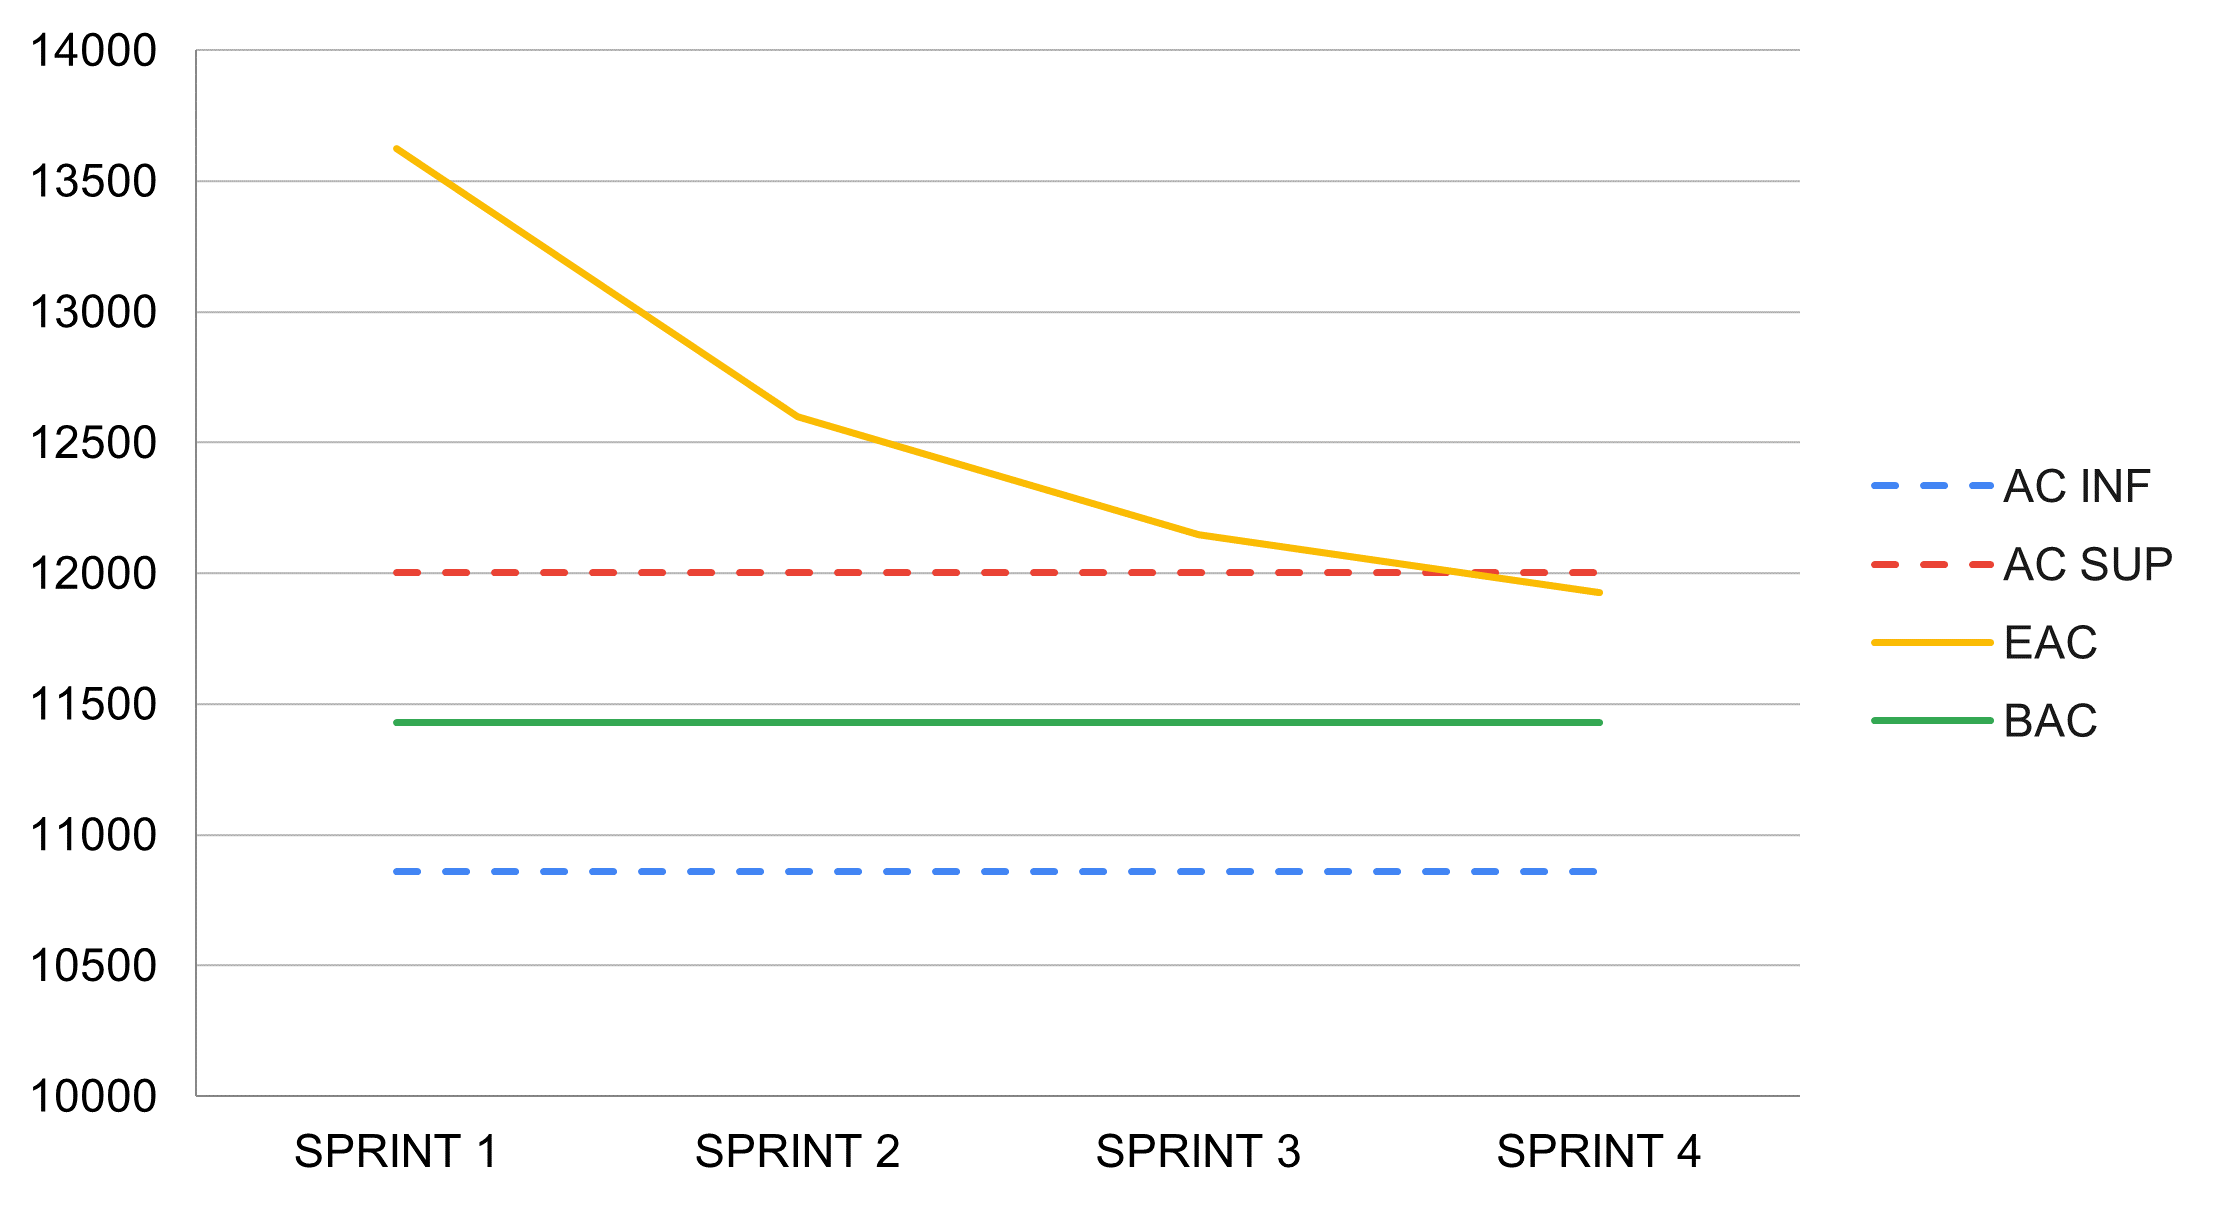
\includegraphics[width=1\textwidth]{images/EAC.png}
    \caption{Proiezione grafica di EAC.}
    \label{fig:Proiezione grafica di EAC}
\end{figure}
\textbf{\glossterm{RTB}:} EAC indica, per ogni periodo, la stima del budget finale prefiguratasi rispetto al valore pianificato definito dal BAC ovvero il Budget at Completion. Questo valore viene calcolato come il rapporto tra BAC e CPI dove CPI è Cost Performance Index.\\
Risulta evidente come la metrica in questione non rientrasse all'interno dei valori di accettazione già dal primo \glossterm{Sprint}. Ciò è dovuto alla scarsa esperienza del team nell'affrontare la pianificazione degli \glossterm{Sprint} e all'altrettanto poca conoscenza rigaurdante le attività prioritarie al fine di una buona gestione del progetto. Negli sprint successivi il team ha preso provvedimenti, adottando con maggiore accortezza una pianificazione efficace e adoperando un metodo lavorativo atto a far rientrare l'EAC all'interno dei valori di accettazione, mantenendo alta, al contempo, la produttività.\\
Il gruppo può trarre esperienza dalla proiezione rappresentata nel grafico in previsione della seconda revisione, mantenendo l'andamento già individuato dal quarto \glossterm{Sprint}.
\clearpage
\subsubsection{MPC-EV Earned Value e MPC-PV Planned Value}
\begin{figure}[h!]
    \centering
    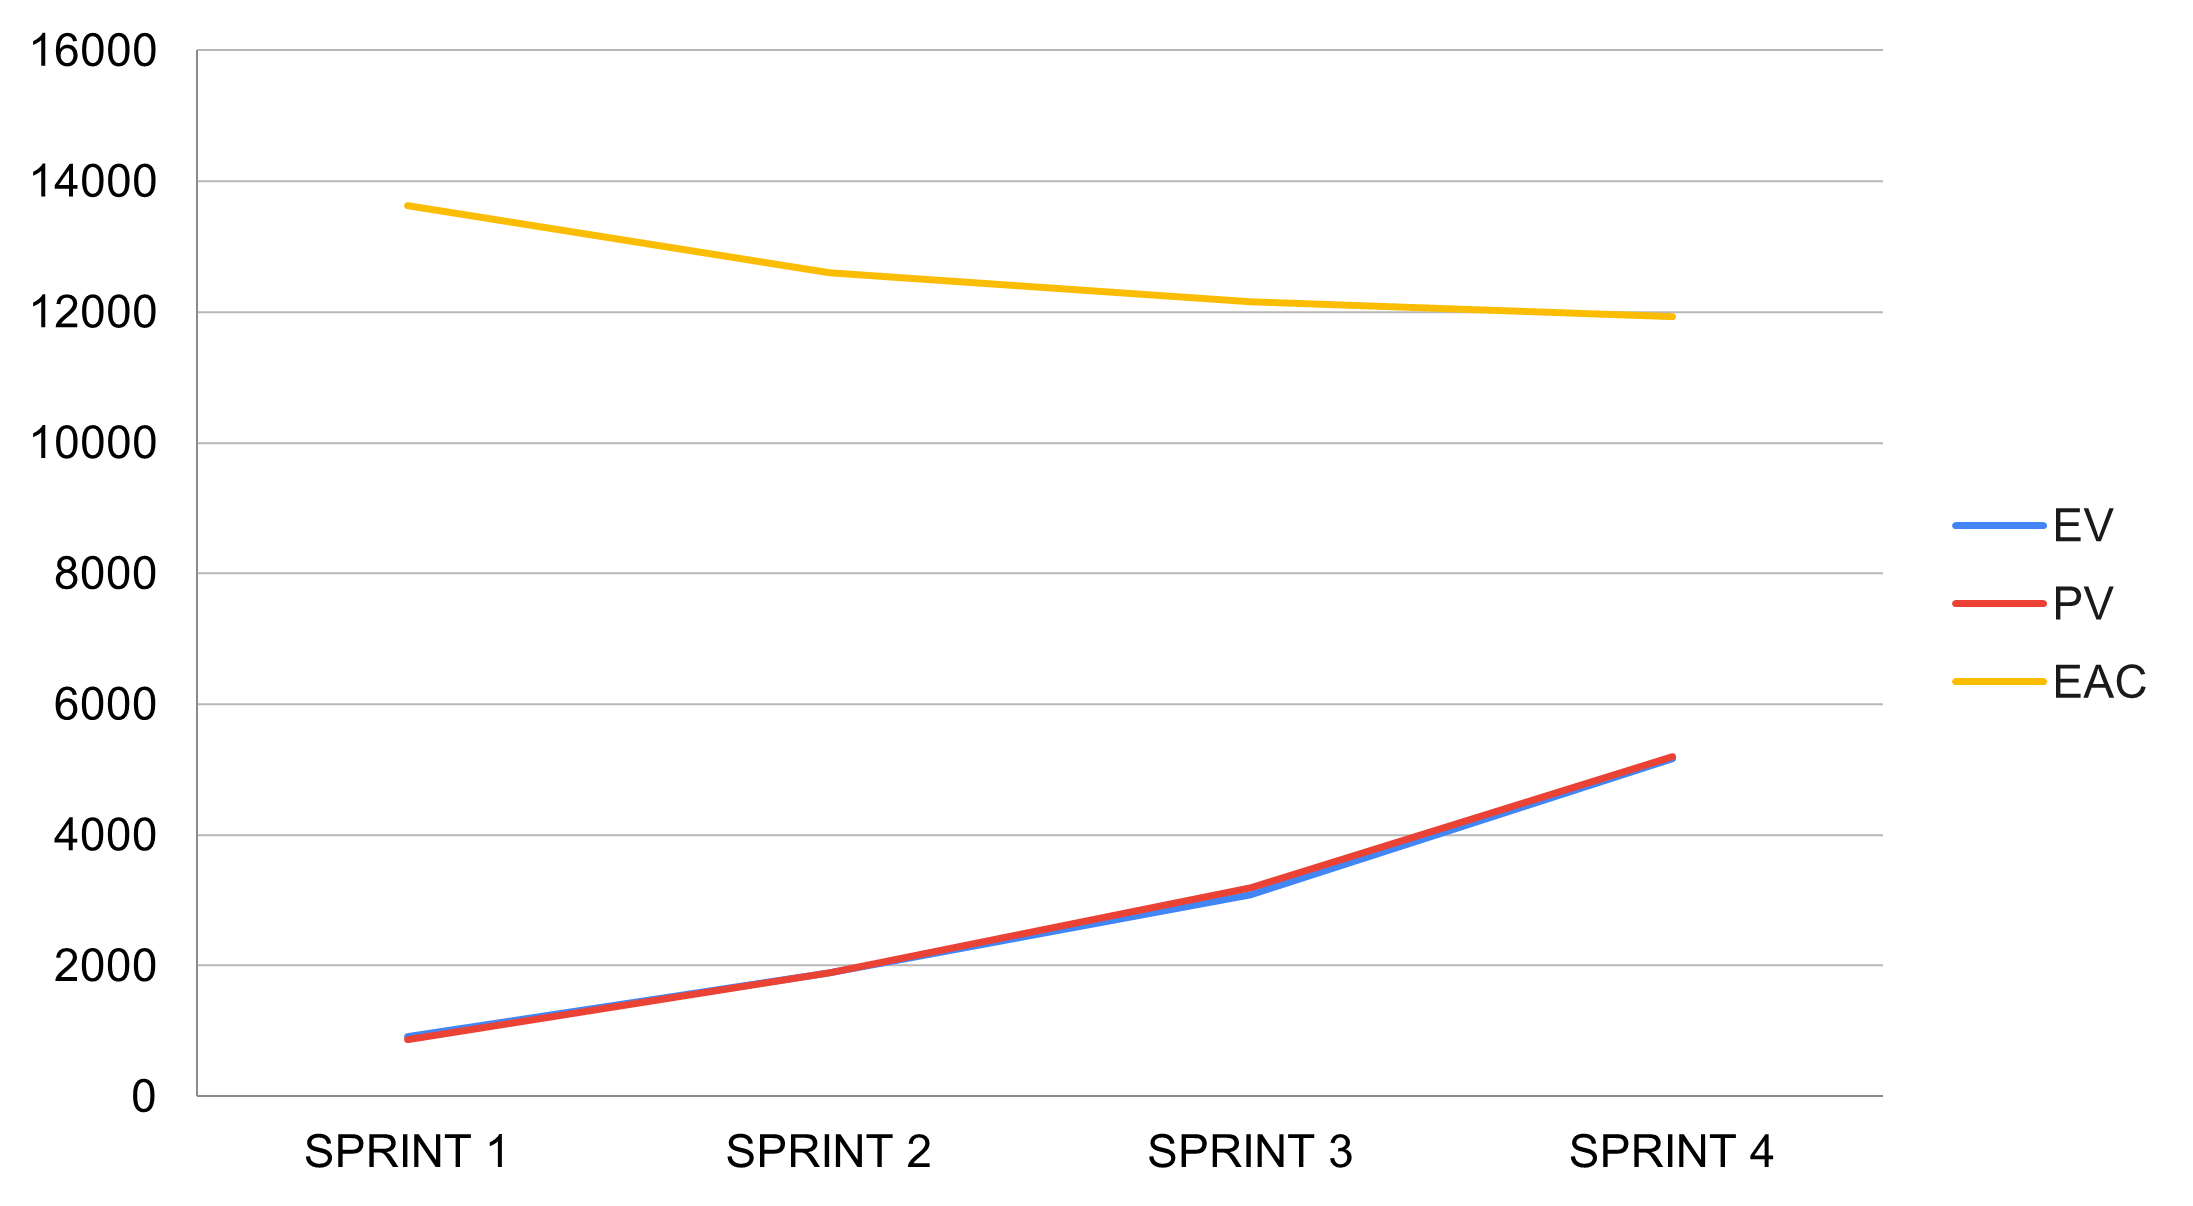
\includegraphics[width=1\textwidth]{images/EV_PV.png}
    \caption{Proiezione grafica di EV e PV.}
    \label{fig:Proiezione grafica di EV e PV}
\end{figure}
\textbf{\glossterm{RTB}:} EV rappresenta il valore generato dal prodotto sviluppato fino a un dato momento mentre PV costituisce il valore del lavoro pianificato fino a un dato momento. Il loro confronto permette di comprendere lo scostamento che avviene tra i preventivi e i consuntivi di lavoro effettuati e quindi ottenere una chiara visione dell'andamento del lavoro svolto dal team.\\
L'andamento delle due metriche è pressoché coincidente, come dimostrato anche nel grafico successivo dalla metrica SV. Dal secondo periodo in poi il valore EV è generalmente inferiore al SV segnalando che il team ha effettuato preventivi ottimistici rispetto all'effettivo risultato prodotto. Ciononostante questa differenza è minimale.
\clearpage
\subsubsection{MPC-BV Budget Variance e MPC-SV Schedule Variance}
\begin{figure}[h!]
    \centering
    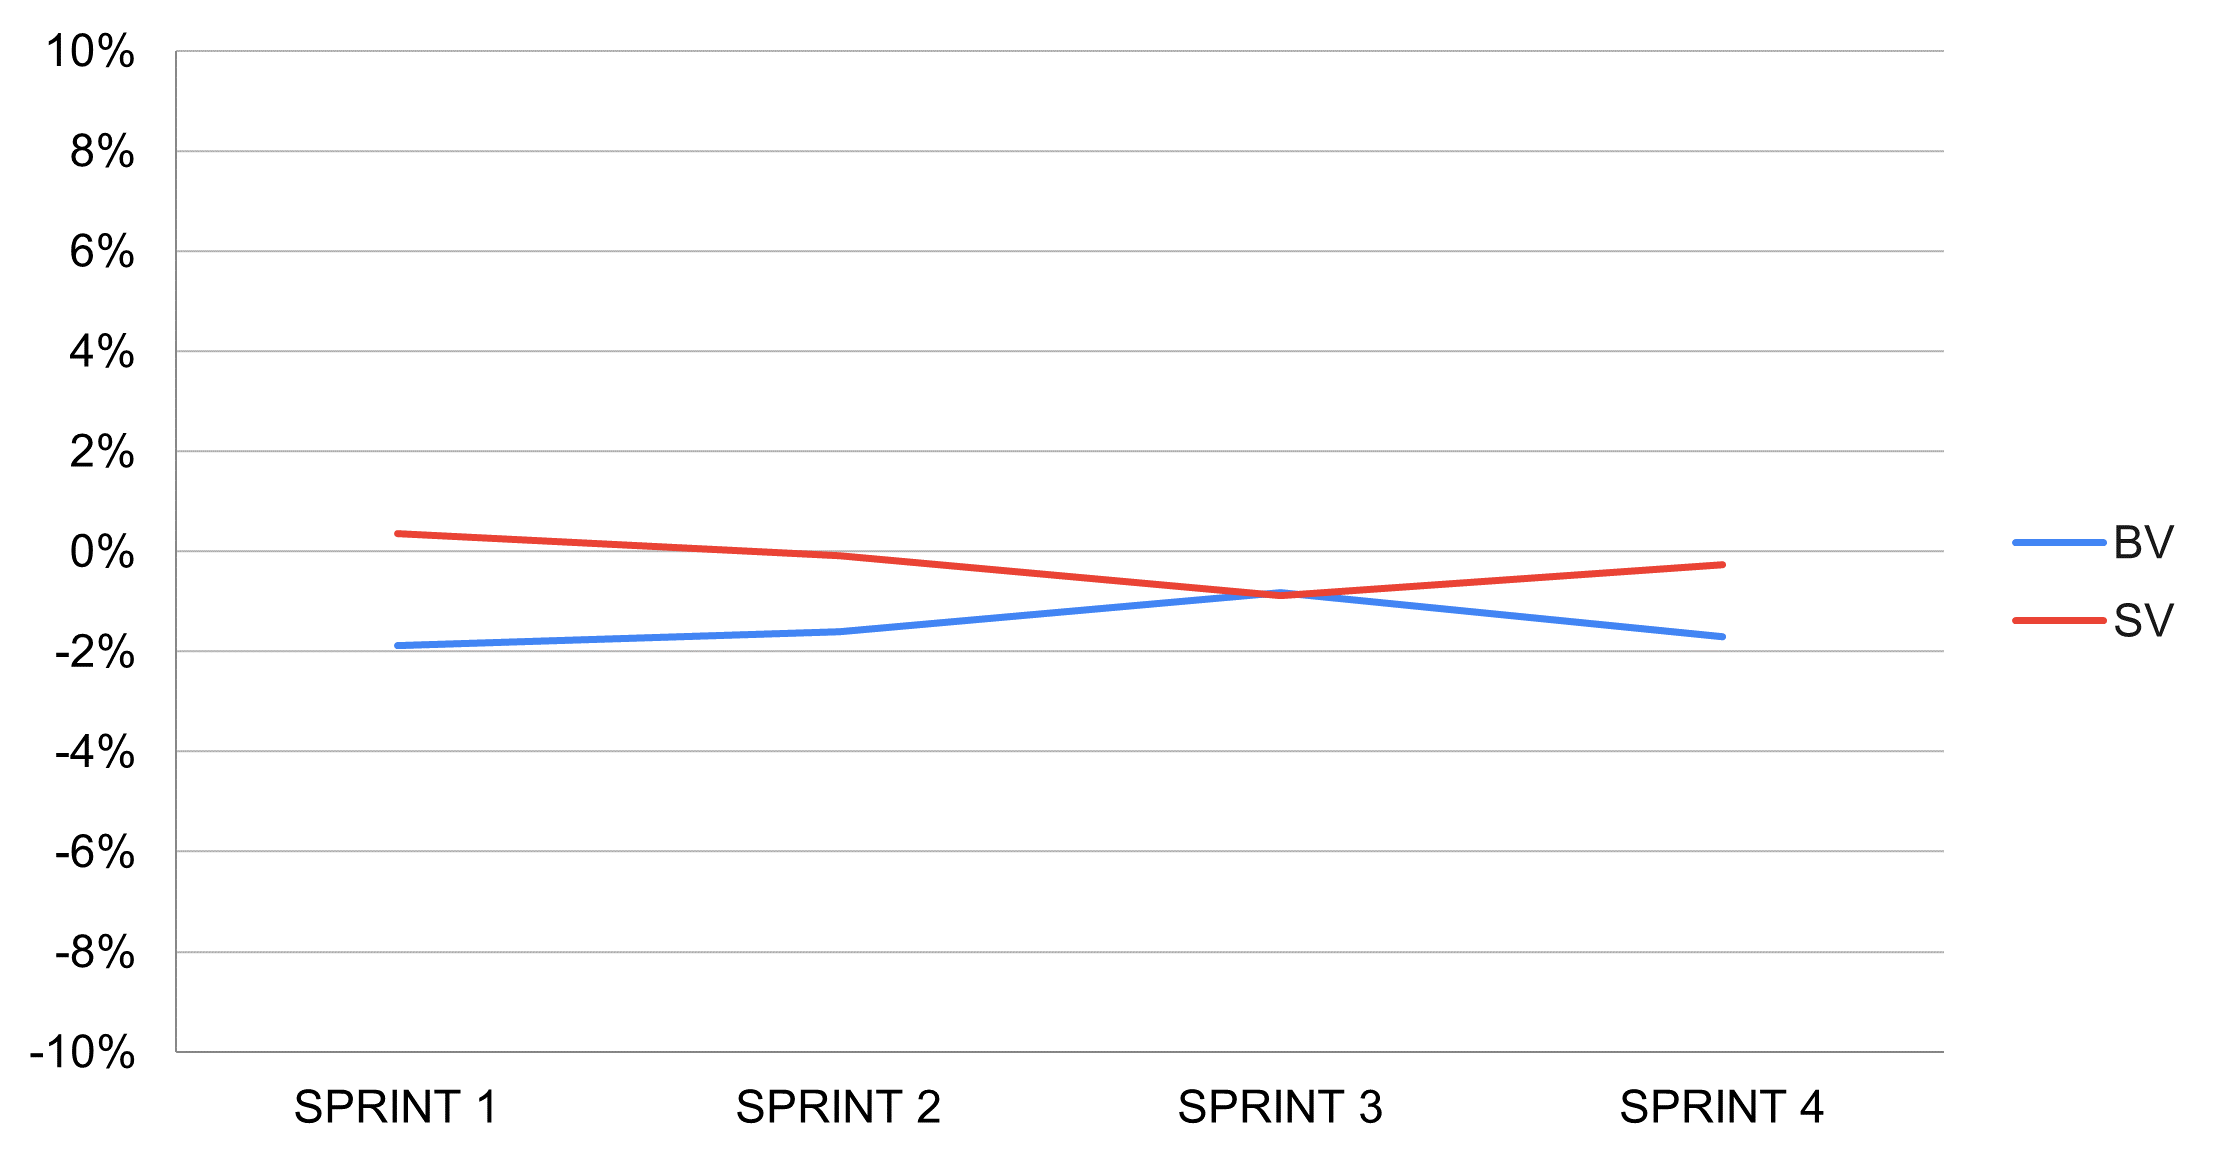
\includegraphics[width=1\textwidth]{images/BV_SV.png}
    \caption{Proiezione grafica di BV e SV.}
    \label{fig:Proiezione grafica di BV e SV}
\end{figure}
\textbf{\glossterm{RTB}:} BV consiste nella differenza tra il valore guadagnato (EV) e i costi effettivamente sostenuti (AC). Un valore negativo di BV indica che si sta spendendo più di quanto si stia guadagnando. SV, invece, rappresenta la differenza tra il valore guadagnato (EV) e il valore pianificato (PV). Un valore negativo indica un ritardo rispetto alla produzione e consegna del lavoro preventivato.\\
Il valore del BV, nonostante sia certamente all'interno dei valori di accettazione, si è mantenuto costantemente negativo dimostrando come i costi effettivamente sostenuti eccedano il lavoro prodotto. Come anticipato nella proiezione dell'EAC, ciò è dovuto alla scarsa esperienza nella pianificazione di preventivi plausibili.\\
La SV ha mantenuto valori oscillanti intorno allo 0, indice di una pianificazione abbastanza realistica rispetto al valore effettivamente prodotto.\\
In generale queste due metriche mantengono valori altamente accettabili sospingendo il team a non deviare dal percorso individuato.
\clearpage
\subsubsection{MPC-AC Actual Cost e MPC-ETC Estimate To Complete}
\begin{figure}[h!]
    \centering
    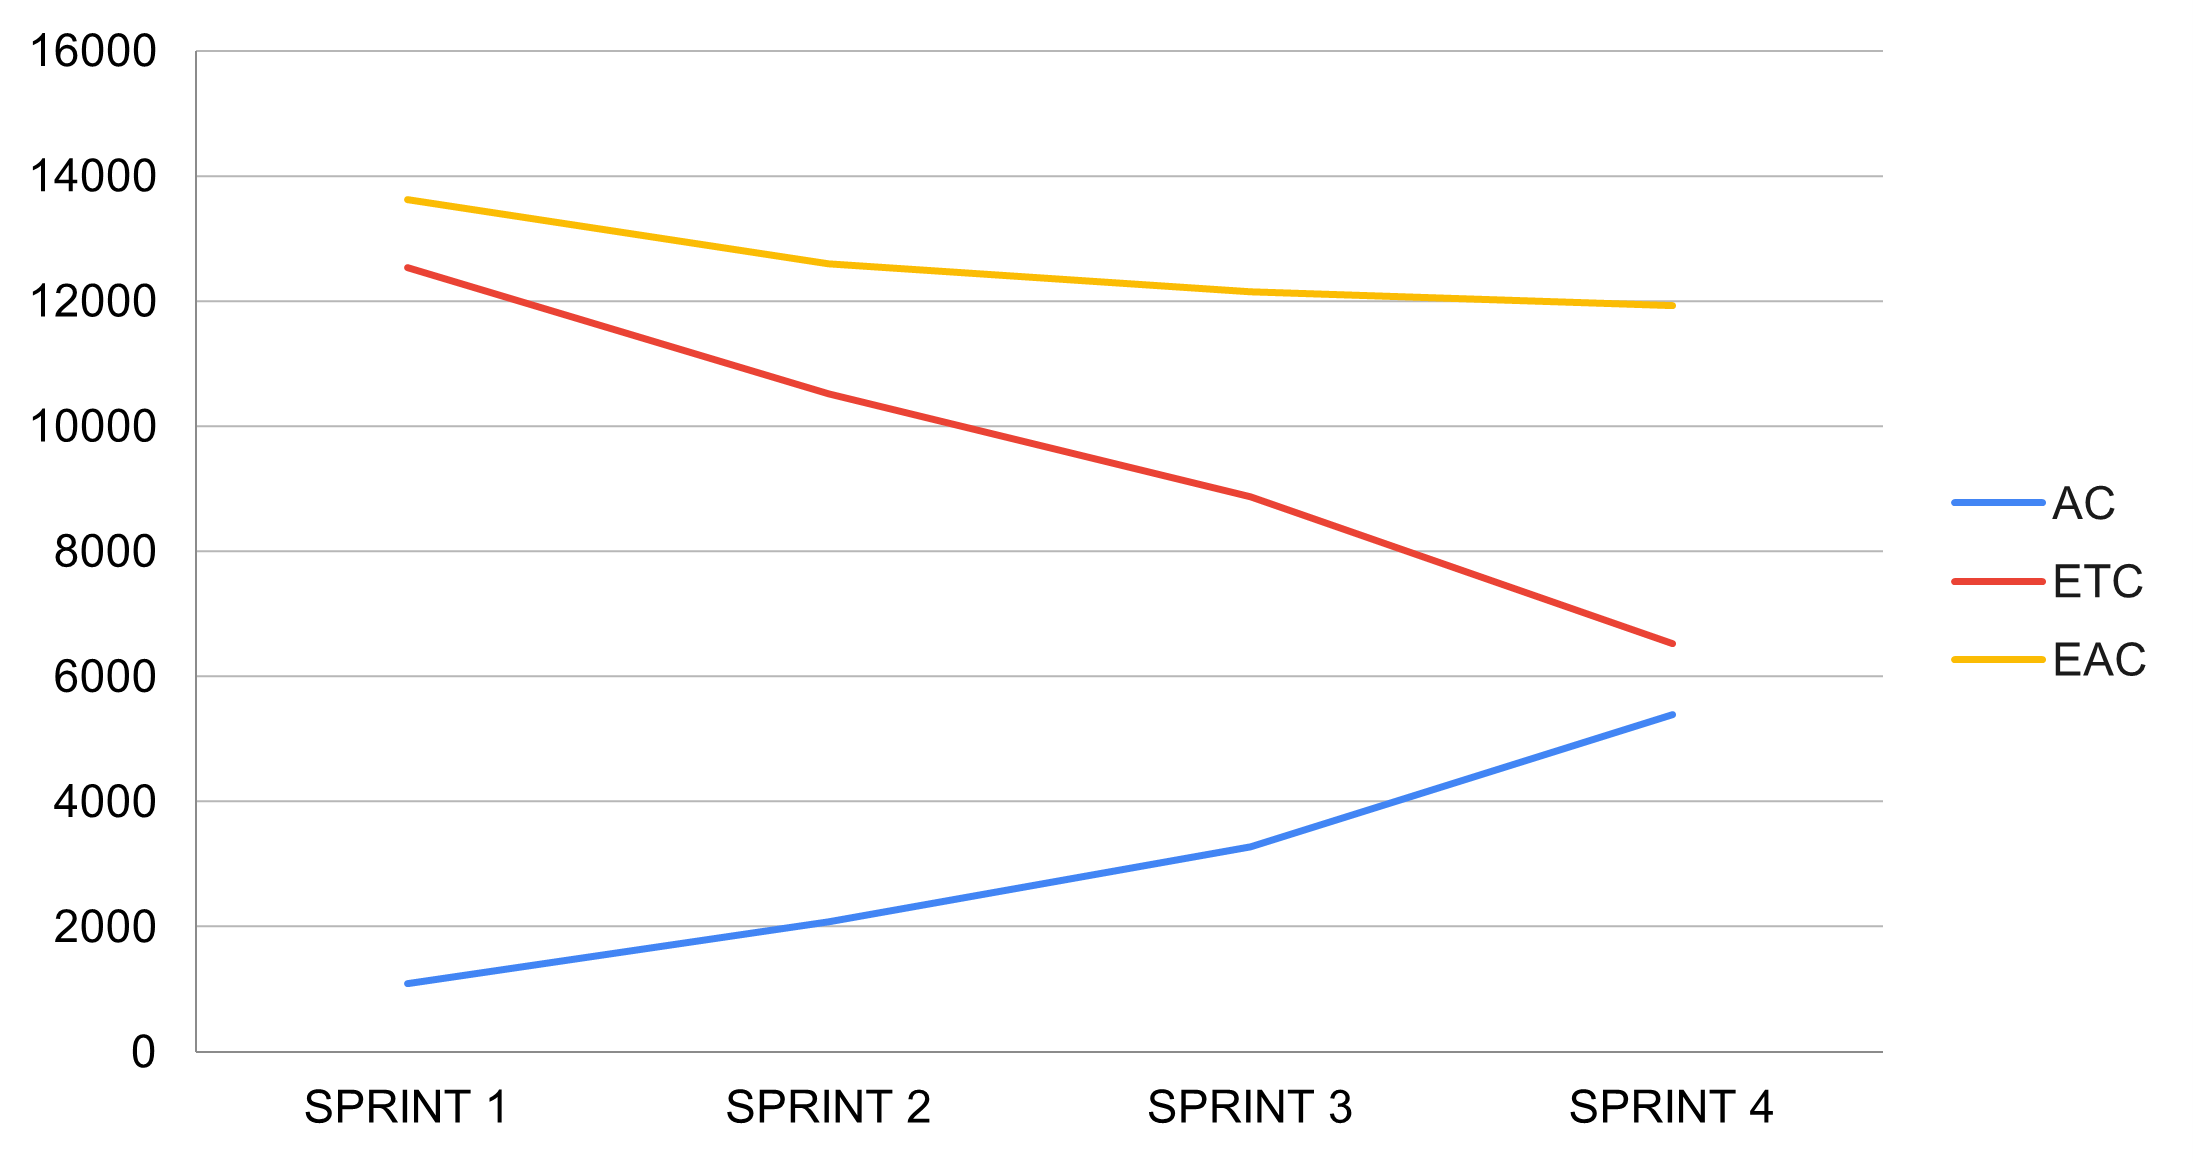
\includegraphics[width=1\textwidth]{images/ETC_AC.png}
    \caption{Proiezione grafica di AC e ETC.}
    \label{fig:Proiezione grafica di AC e ETC}
\end{figure}
\textbf{\glossterm{RTB}:} AC rappresenta il costo sostenuto fino a un dato momento mentre ETC consiste nella conseguente stima dei costi da sostenere per il completamento del progetto.\\
Totalmente in linea con quanto rilevato dalla proiezione delle metriche di EAC, BV e SV, l'AC e l'ETC dimostrano l'avanzamento stimato del progetto. I quattro \glossterm{Sprint} rappresentati corrispondono all'arco di tempo definito da 9 settimane, corrispondenti a circa metà del progetto. Ci si aspetta quindi che le due metriche siano prossime ad incontrarsi, considerando un lieve ritardo rispetto alla pianificazione determinato dal valore leggermente negativo di SV.
\clearpage
\subsubsection{MPC-CPI Cost Performance Index}
\begin{figure}[h!]
    \centering
    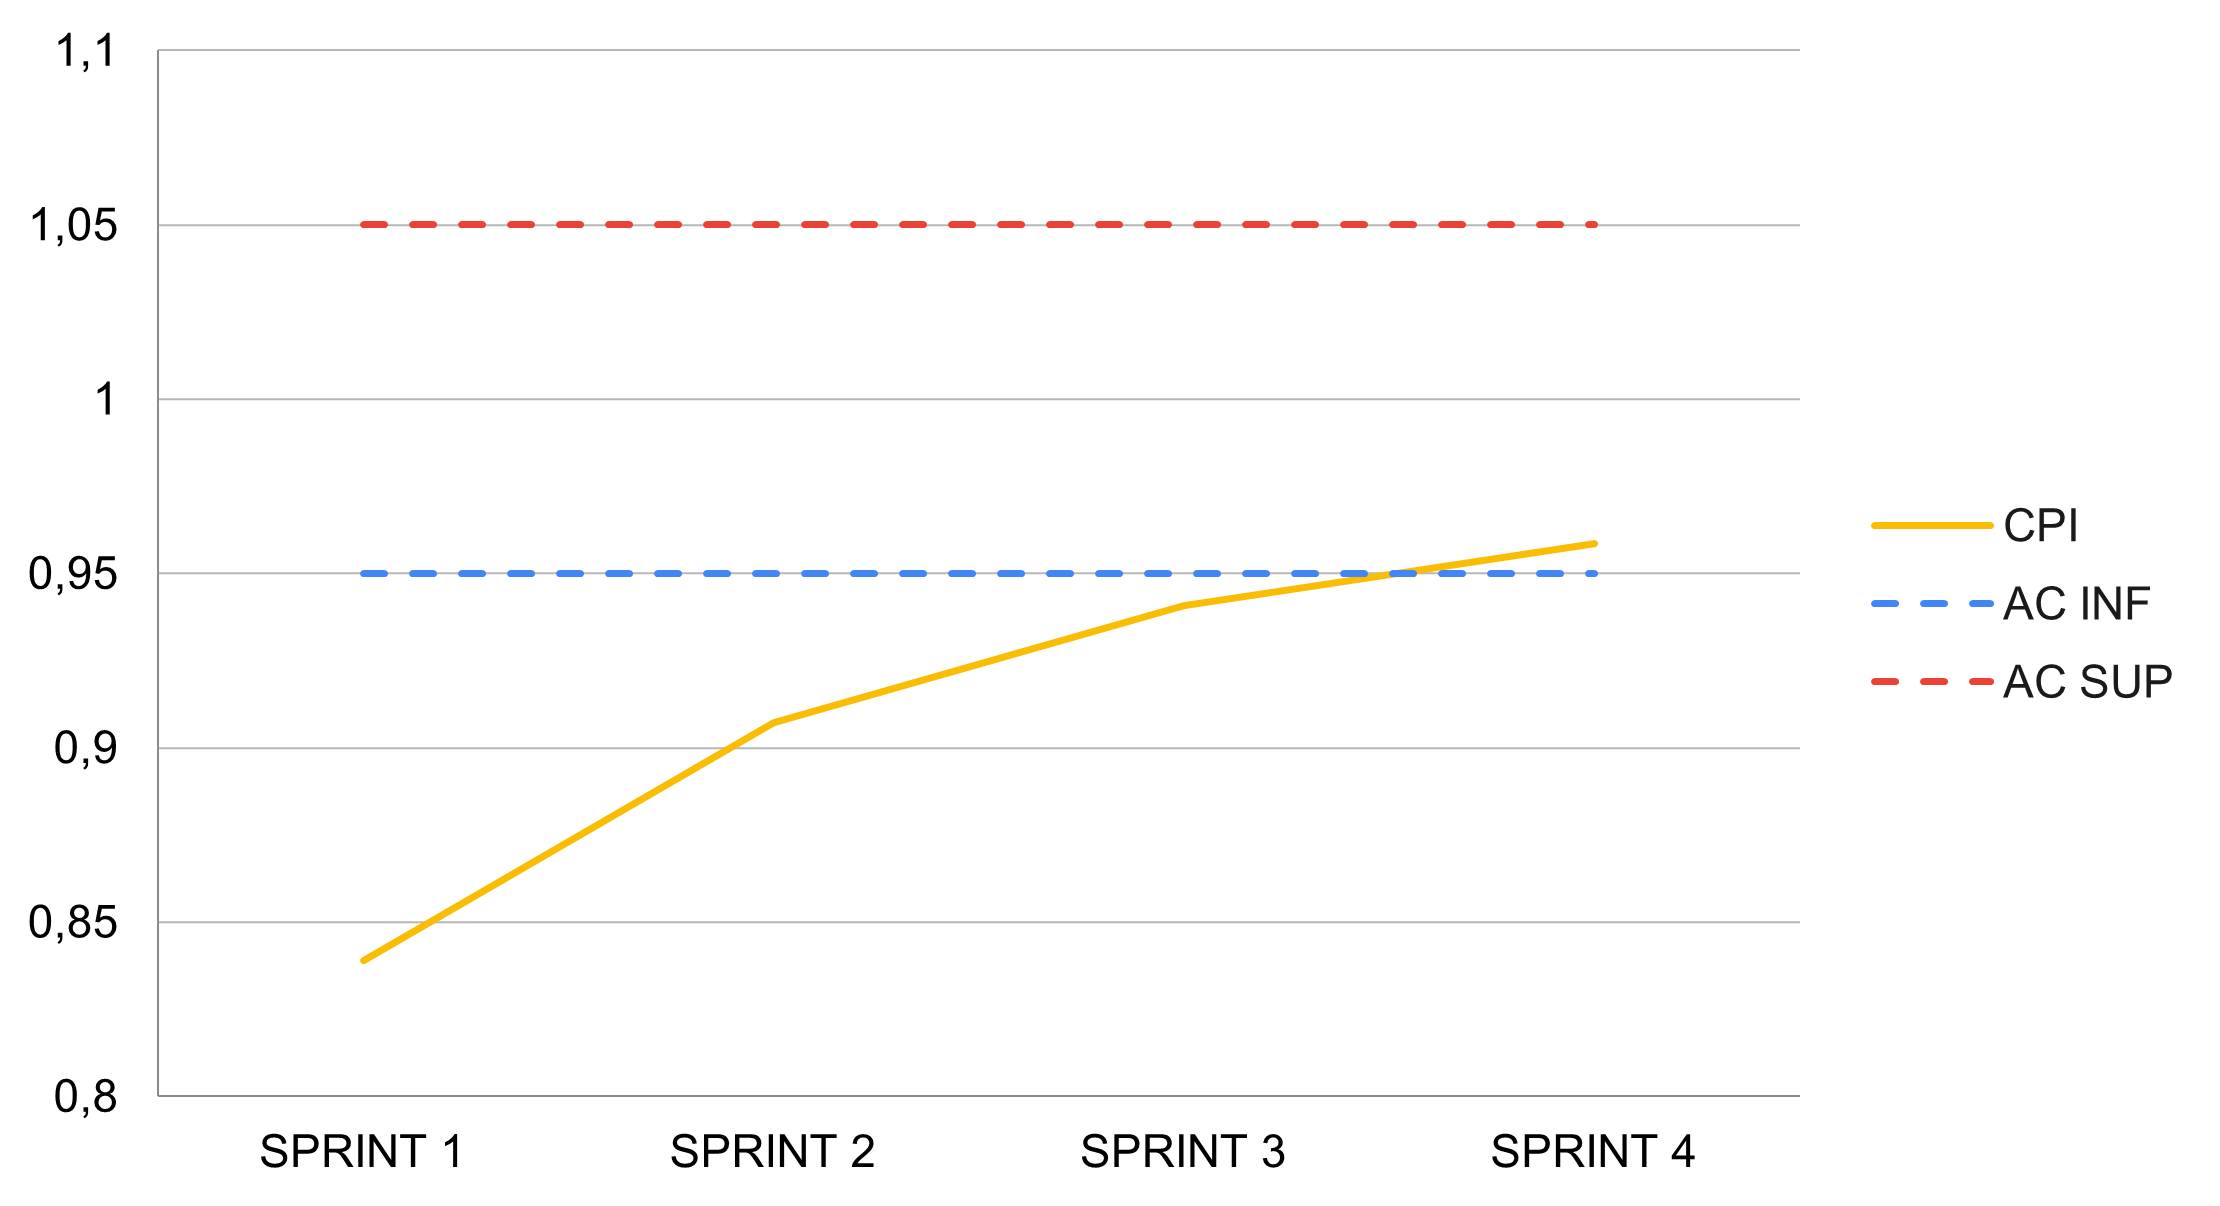
\includegraphics[width=1\textwidth]{images/CPI.png}
    \caption{Proiezione grafica di CPI.}
    \label{fig:Proiezione grafica di CPI}
\end{figure}
\textbf{\glossterm{RTB}:} CPI indica il rapporto tra il valore guadagnato (EV) e i costi sostenuti (AC). Un valore di CPI uguale a 1 indica che i costi sostenuti sono in linea con il bugdet pianificato (BAC) mentre un valore negativo comporta il discostamento della stima del bidget al completamento (EAC) dal budget effettivo.\\
Coerentemente con quanto indicato dall'EAC, il valore di CPI è rimasto al di fuori dei valori di accettazione fino al quarto \glossterm{Sprint}. Specialmente nei primi periodi il team ha sostenuto costi eccessivi non solo rispetto al valore pianificato ma soprattutto rispetto al valore prodotto. Le accortezze adottate negli \glossterm{Sprint} successivi hanno avuto gli effetti desiderati portando il valore di CPI vicino ad 1 e di conseguenza portando ad una diminuzione dell'EAC. Il team si impegna nei prossimi periodi a mantenere l'indice all'interno delle soglie di accettazione.  
\clearpage
\subsubsection{MPC-VAC Variance At Completion}
\begin{figure}[h!]
    \centering
    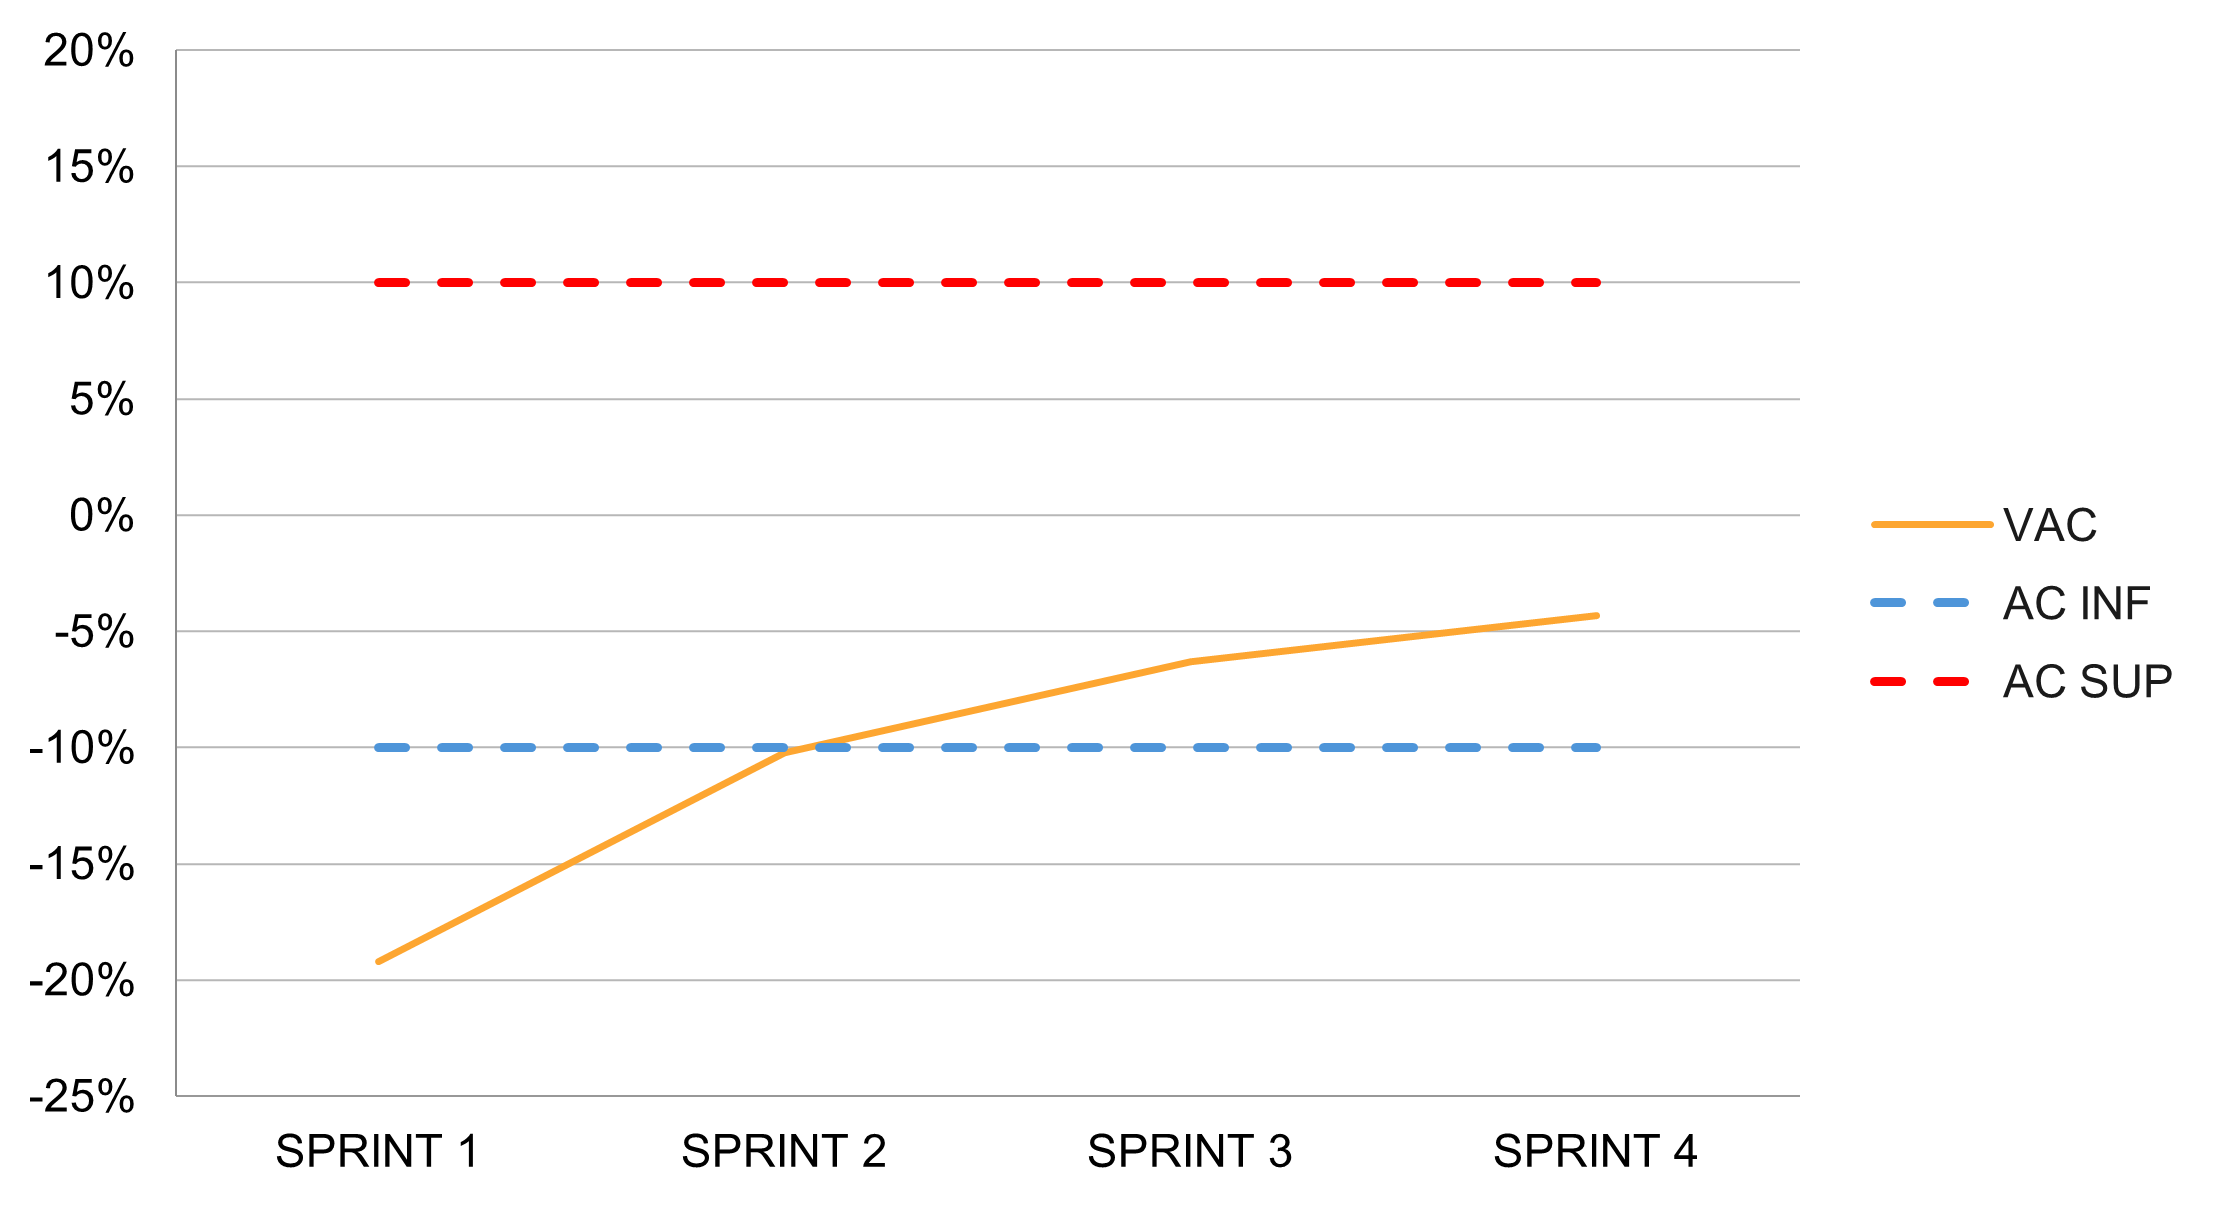
\includegraphics[width=1\textwidth]{images/VAC.png}
    \caption{Proiezione grafica di VAC.}
    \label{fig:Proiezione grafica di VAC}
\end{figure}
\textbf{\glossterm{RTB}:} VAC indica la variazione relativa del budget pianificato, ovvero il BAC, rispetto al budget stimato dall'EAC. L'itervallo di accettazione di questa metrica è posto ad una differenza in percentuale del 10\% rispetto al BAC.\\
Coerentemente con quanto indicato dall'EAC, il valore di VAC è risultato maggiore del -10\% indicando un EAC eccessivamente superiore rispetto al BAC pianificato. Le accortezze adottate negli \glossterm{Sprint} successivi hanno avuto gli effetti desiderati portando il valore di VAC all'interno dell'intervallo di accettazione dal terzo \glossterm{Sprint}.
\clearpage
\subsection{Qualità di processo - Documentazione}
\subsubsection{Indice Gulpease}
\begin{figure}[h!]
    \centering
    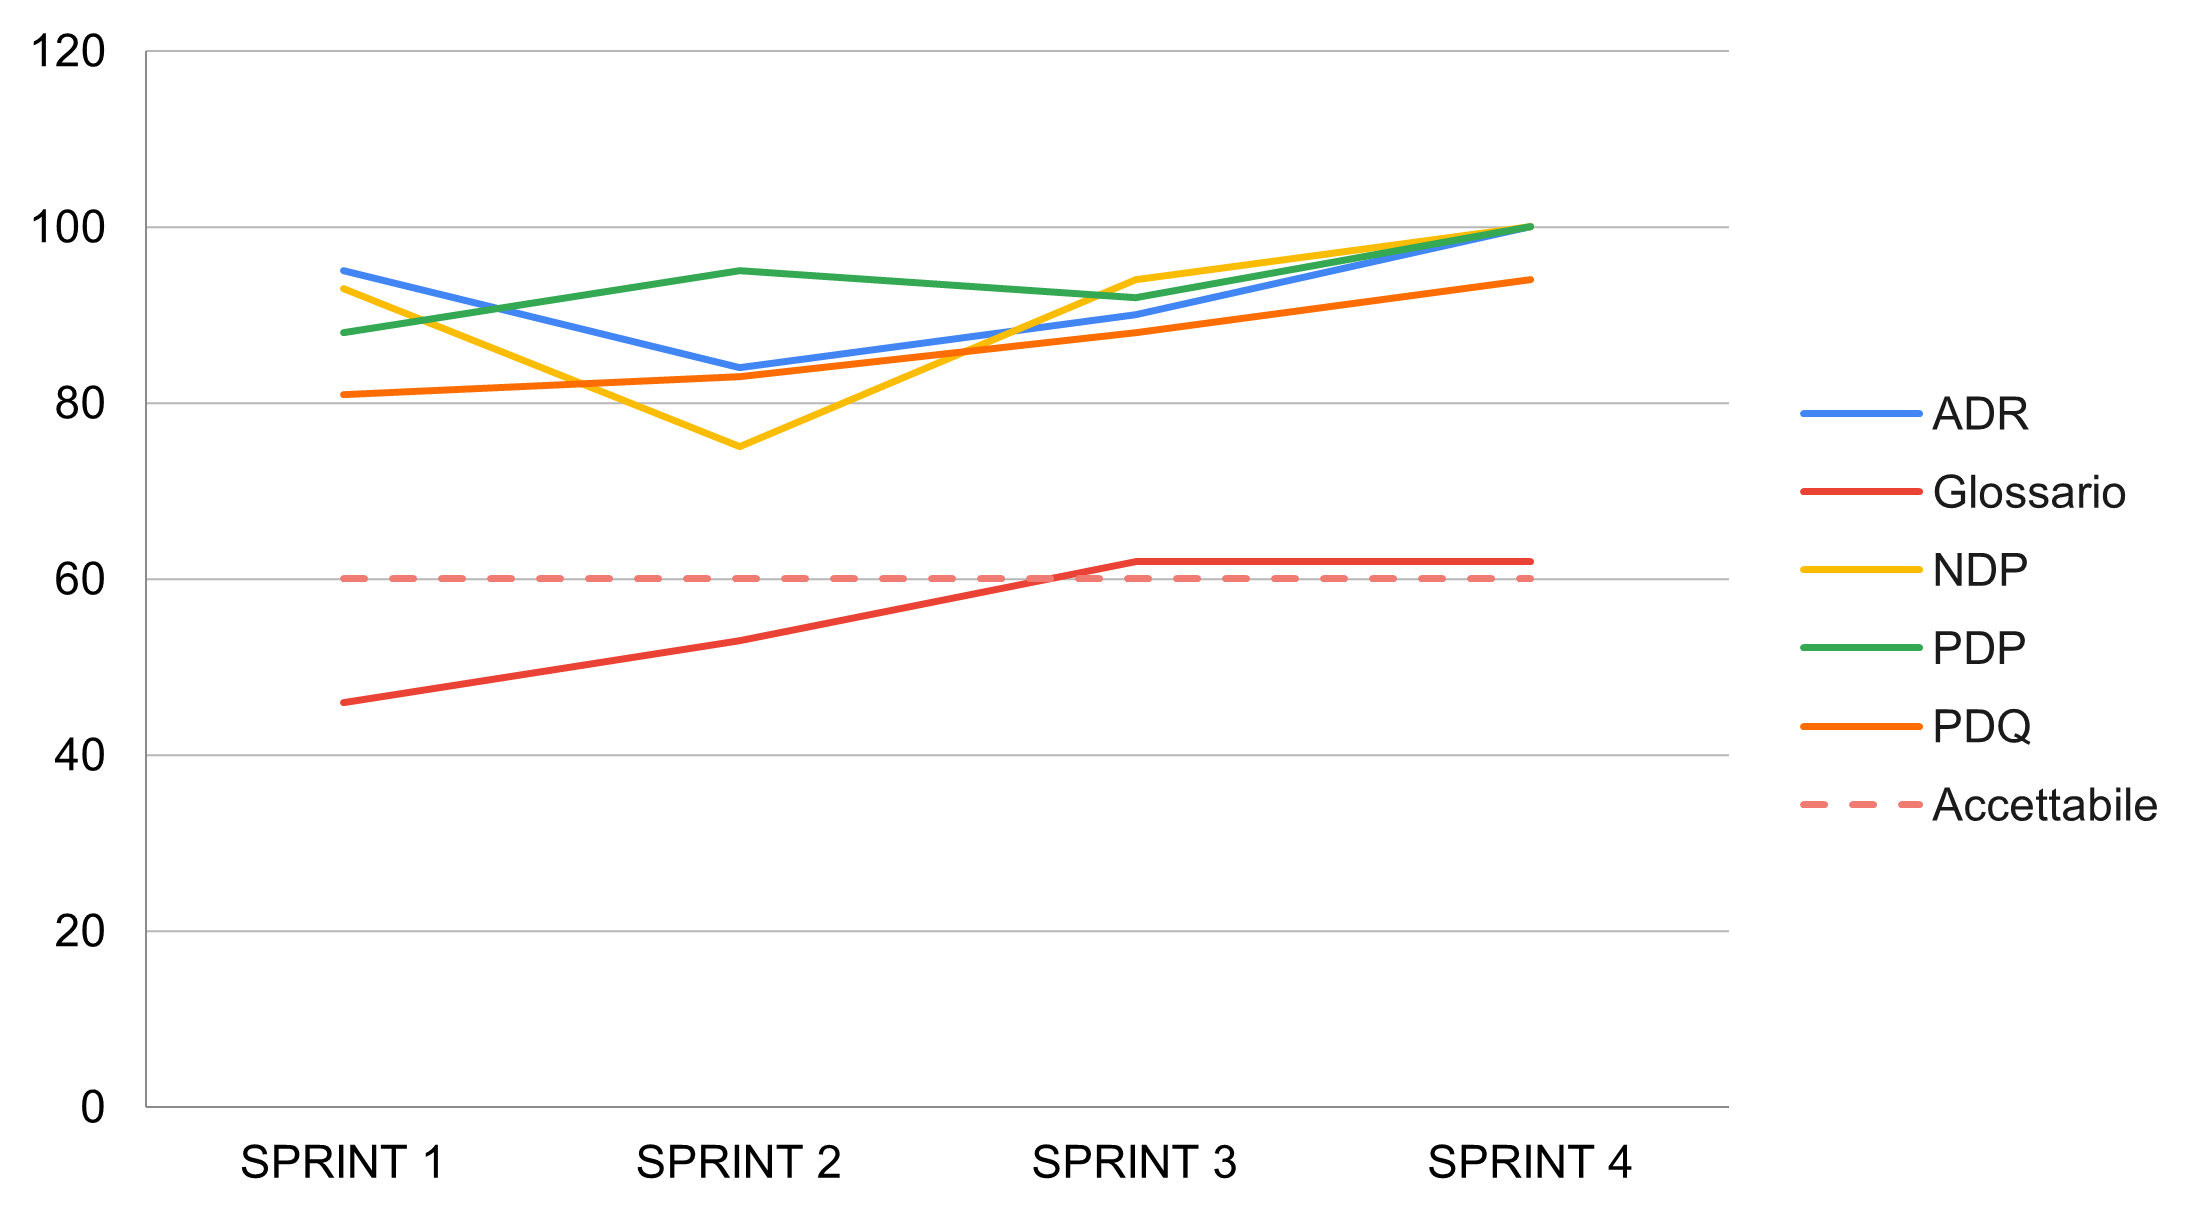
\includegraphics[width=1\textwidth]{images/IG.png}
    \caption{Proiezione grafica dell'indice gulpease.}
    \label{fig:Proiezione grafica dell'indice gulpease}
\end{figure}
\textbf{\glossterm{RTB}:} L'indice Gulpease è un'indice di leggibilità per testi in lingua italiana ed è indicato da una percetuale di leggibilità, con soglia di accettazione al 60\%. Tutti i documenti prodotti dal team hanno prodotto un indice di leggibilità alto e nella maggior parte anche ottimale. L'unica eccezione si individua nel \textit{Piano di Qualifica} ma sopratutto nel \textit{Glossario} che fino all'ultimo ha avuto valori inferiori alla soglia di accettazione. Nonostante ciò, sarà di fondamentale importanza per il team migliorare l'indice di leggibilità di questo documento.
\clearpage
\subsubsection{Correttezza Ortografica}
\begin{figure}[h!]
    \centering
    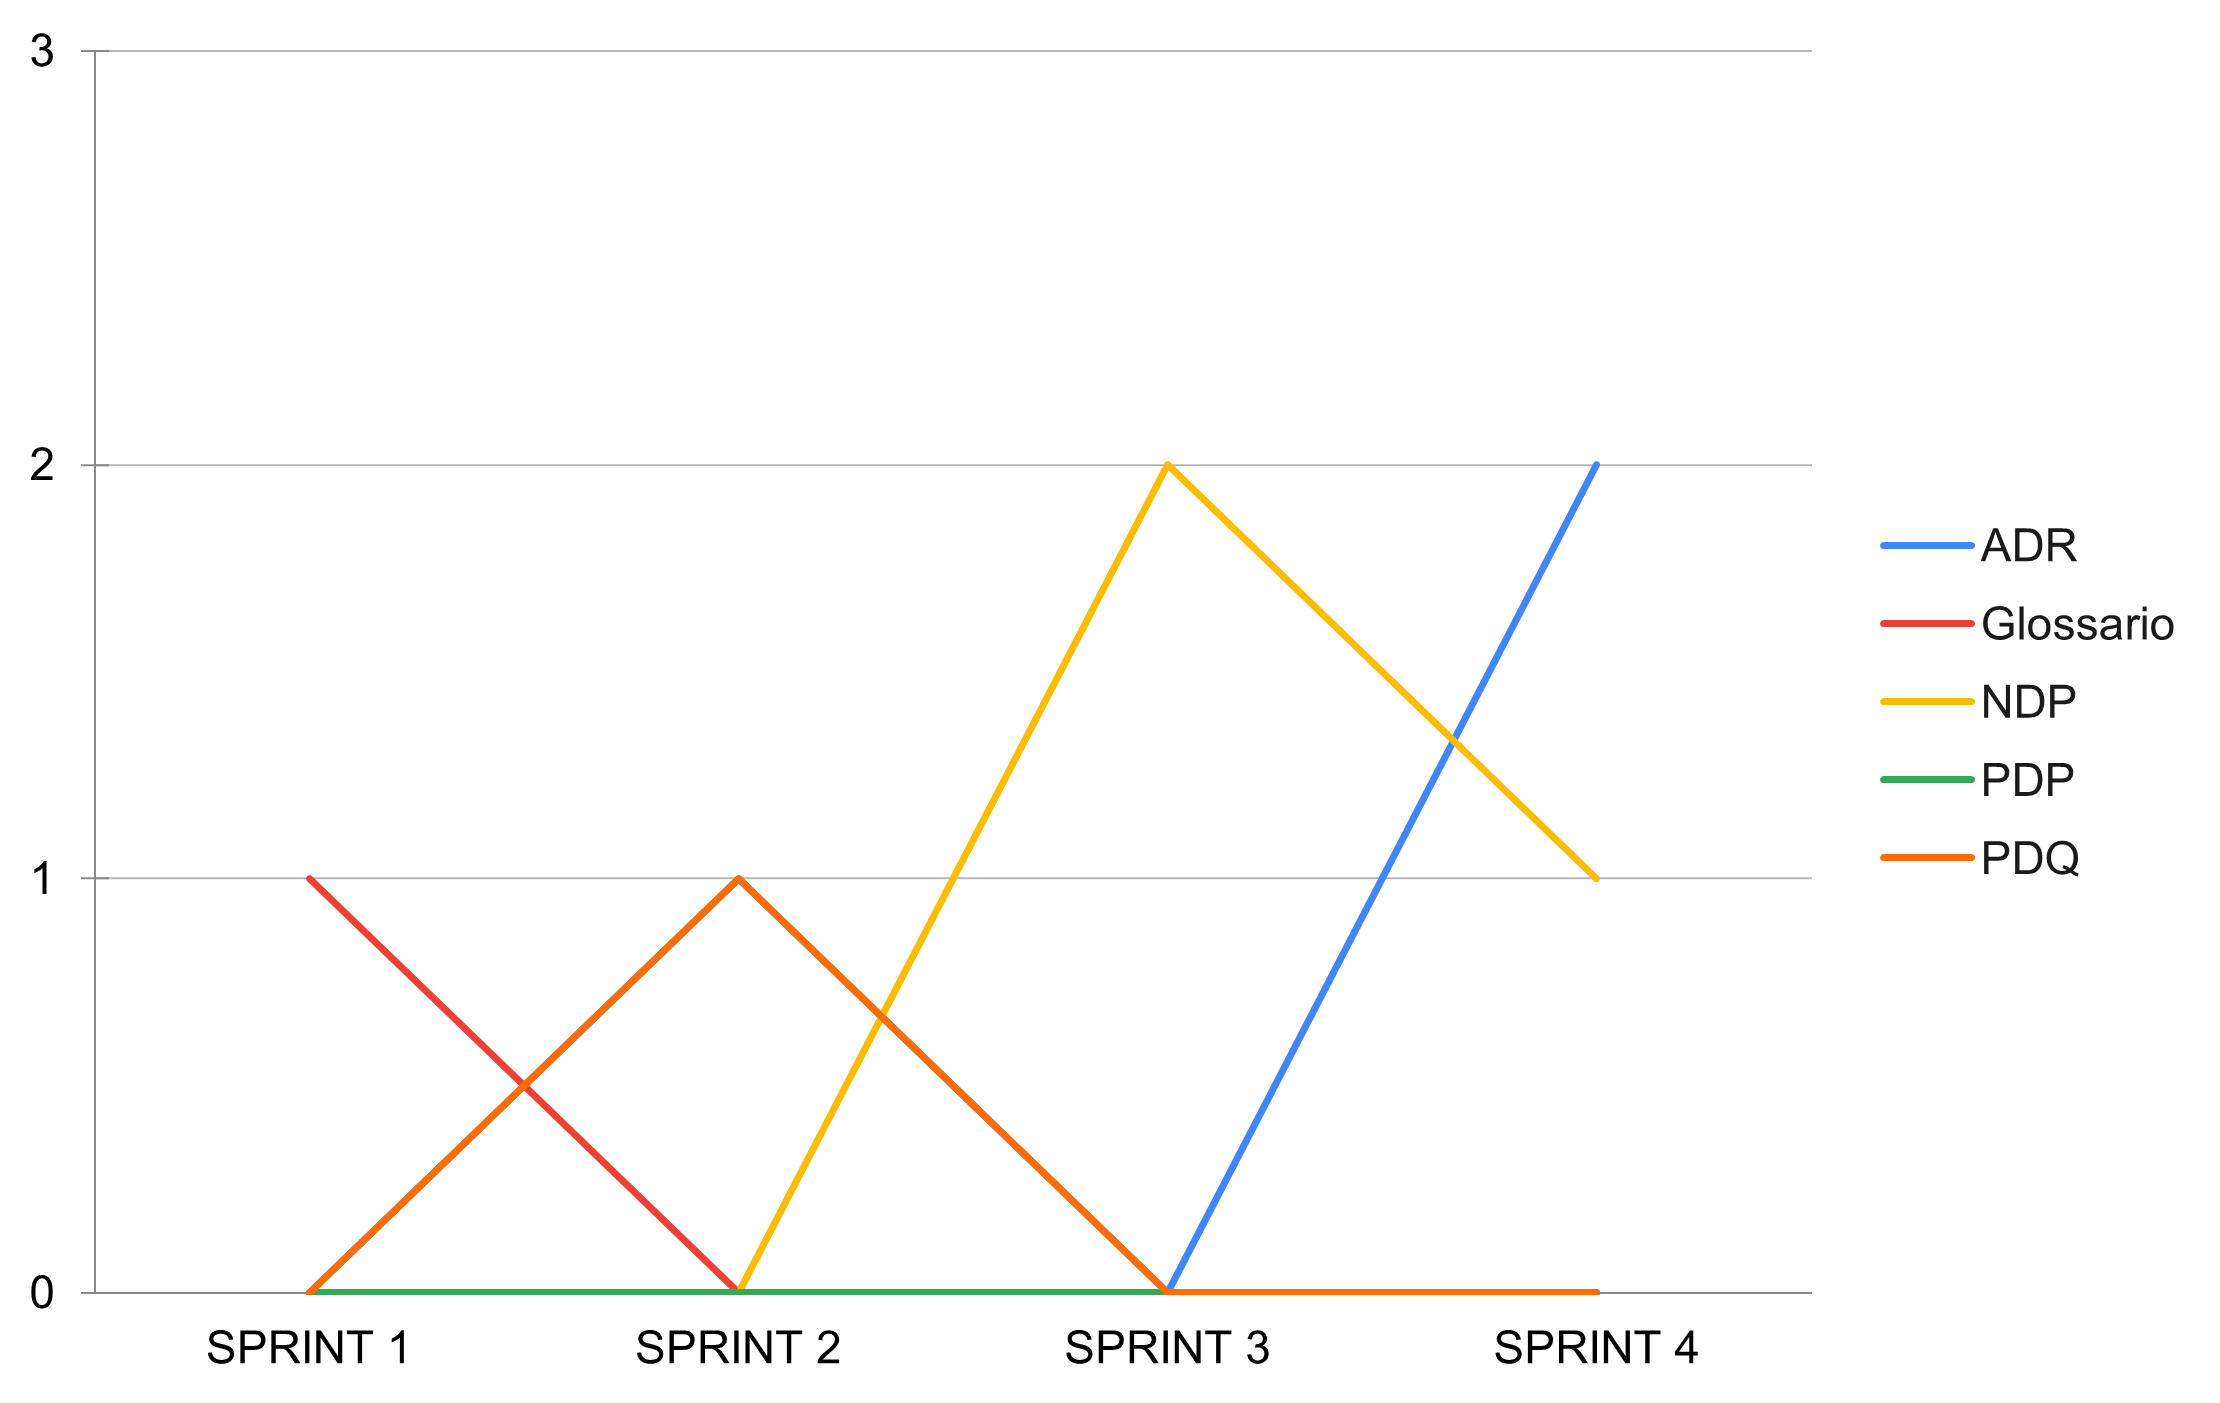
\includegraphics[width=1\textwidth]{images/CO.png}
    \caption{Proiezione grafica della correttezza ortografica.}
    \label{fig:Proiezione grafica della correttezza ortografica}
\end{figure}
\textbf{\glossterm{RTB}:} Il team ha costantemente effettuato un controllo approfondito della correttezza ortografica dei documenti prodotti. I redattori hanno il compito di assicurarsene prima ancora della verifica del documento da parte di terzi membri. Successivamente in vista delle revisione questi vengono ricontrollati e approvati. In questo modo ogni documento viene sempre visionato e controllato da ogni membro del gruppo ottenendo come risultato un esiguo numero di errori e, di conseguenza, l'ottima proiezione rappresentata.
\clearpage
\subsection{Qualità di processo - Gestione della qualità}
\subsubsection{MPC-QMS Quality Metrics Satisfied}
\begin{figure}[h!]
    \centering
    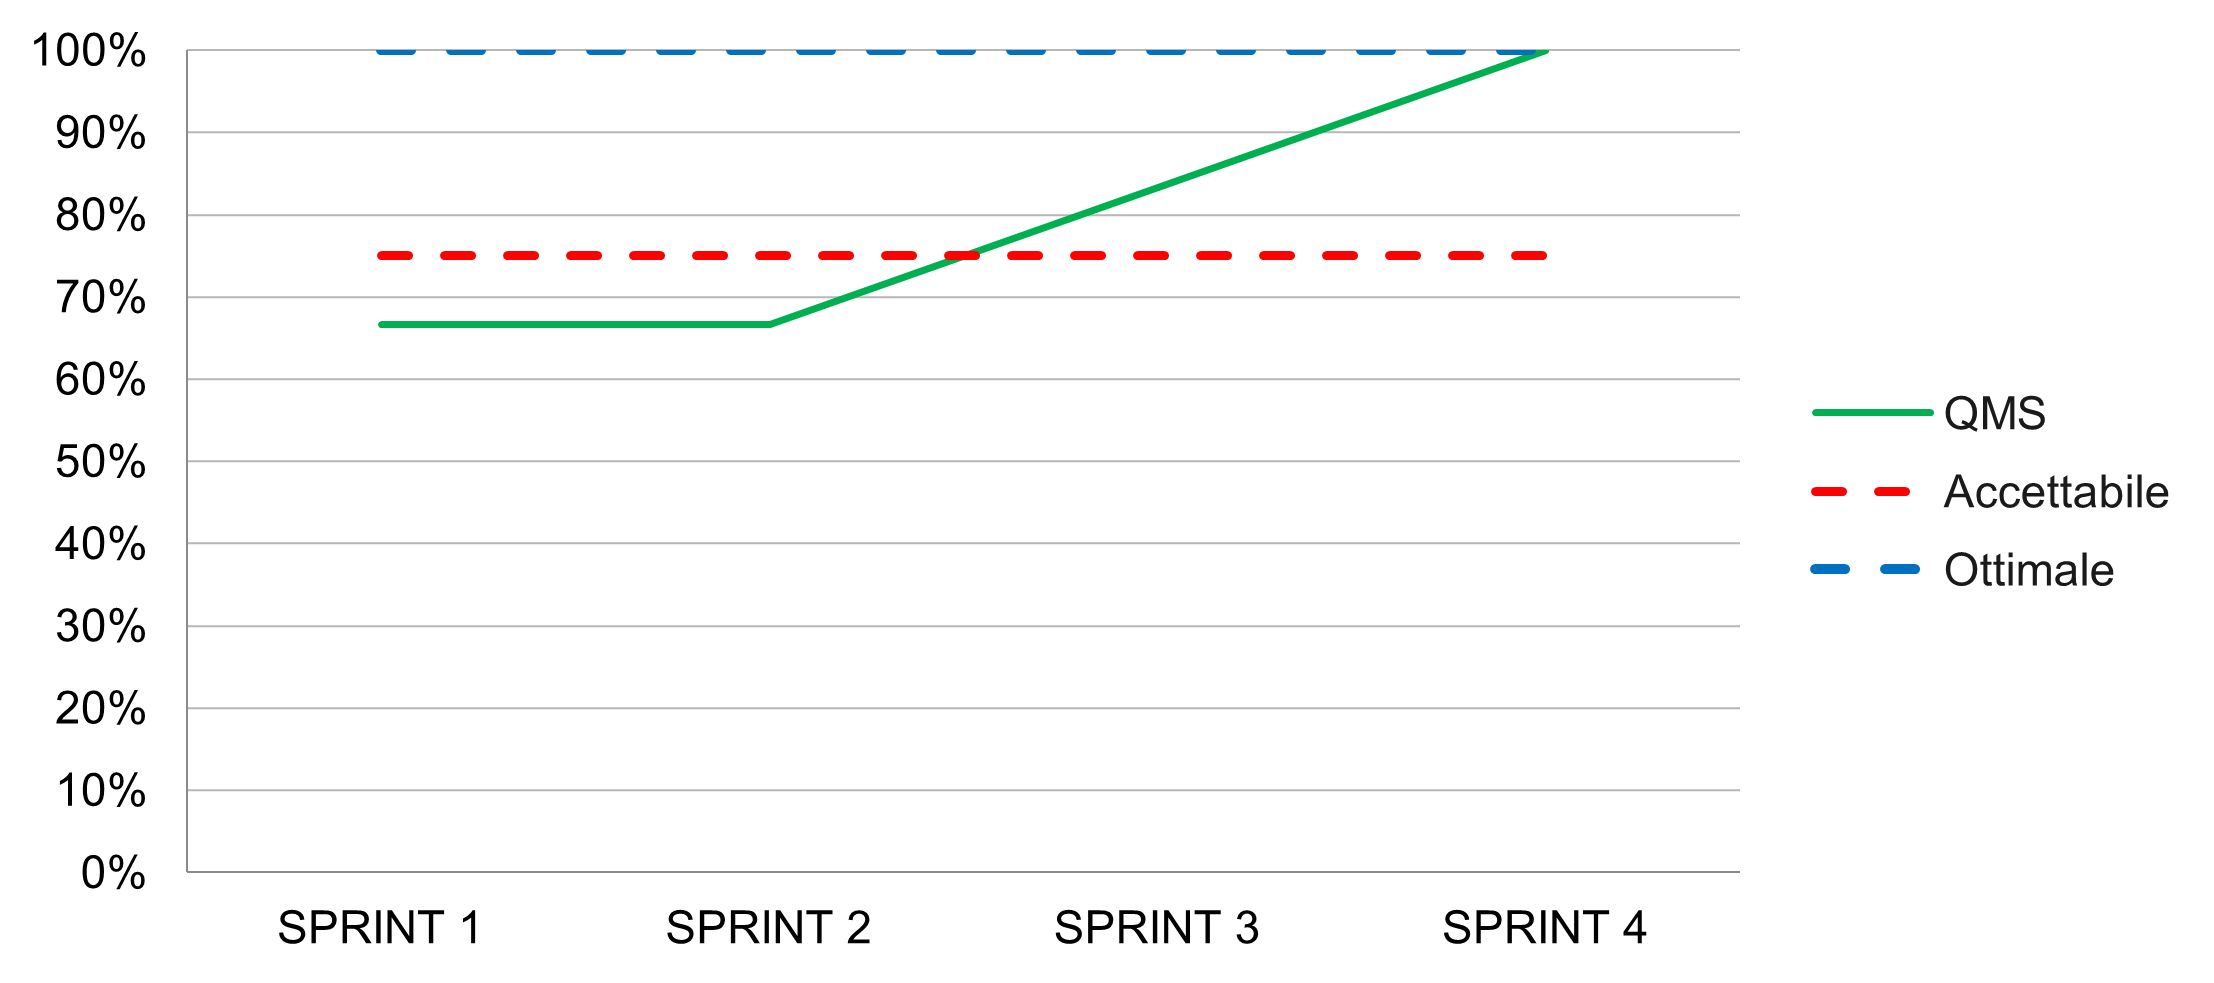
\includegraphics[width=1\textwidth]{images/QMS.png}
    \caption{Proiezione grafica di QMS.}
    \label{fig:Proiezione grafica di QMS}
\end{figure}
\textbf{\glossterm{RTB}:} In linea con quanto già specificato, le metriche di EAC, CPI, VAC e IG non sono state soddisfatte fin da subito. Il VAC e l'indice Gulpease, in particolare per il \textit{Glossario}, sono rientrati nei valori accettabili solamente dal terzo \glossterm{Sprint}, mentre l'EAC e il CPI dal quarto. Con ottica di retrospettiva il team nota come è stata necessaria l'acquisizione di esperienza e accortezza nella pianificazione e organizzazione delle attività del gruppo, cause primarie della mancata tollerabilità delle metriche citate. Questo non deve distogliere il team dal mantenere l'andamento individuato affiché tutte le metriche vengano rispettate, il prodotto venga sviluppato senza intoppi e il progetto possa essere portato a termine senza imprevisti. 
\clearpage
\subsection{Qualità di processo - Gestione dei processi}
\subsubsection{MPC-NR Non-calculated Risk}
\begin{figure}[h!]
    \centering
    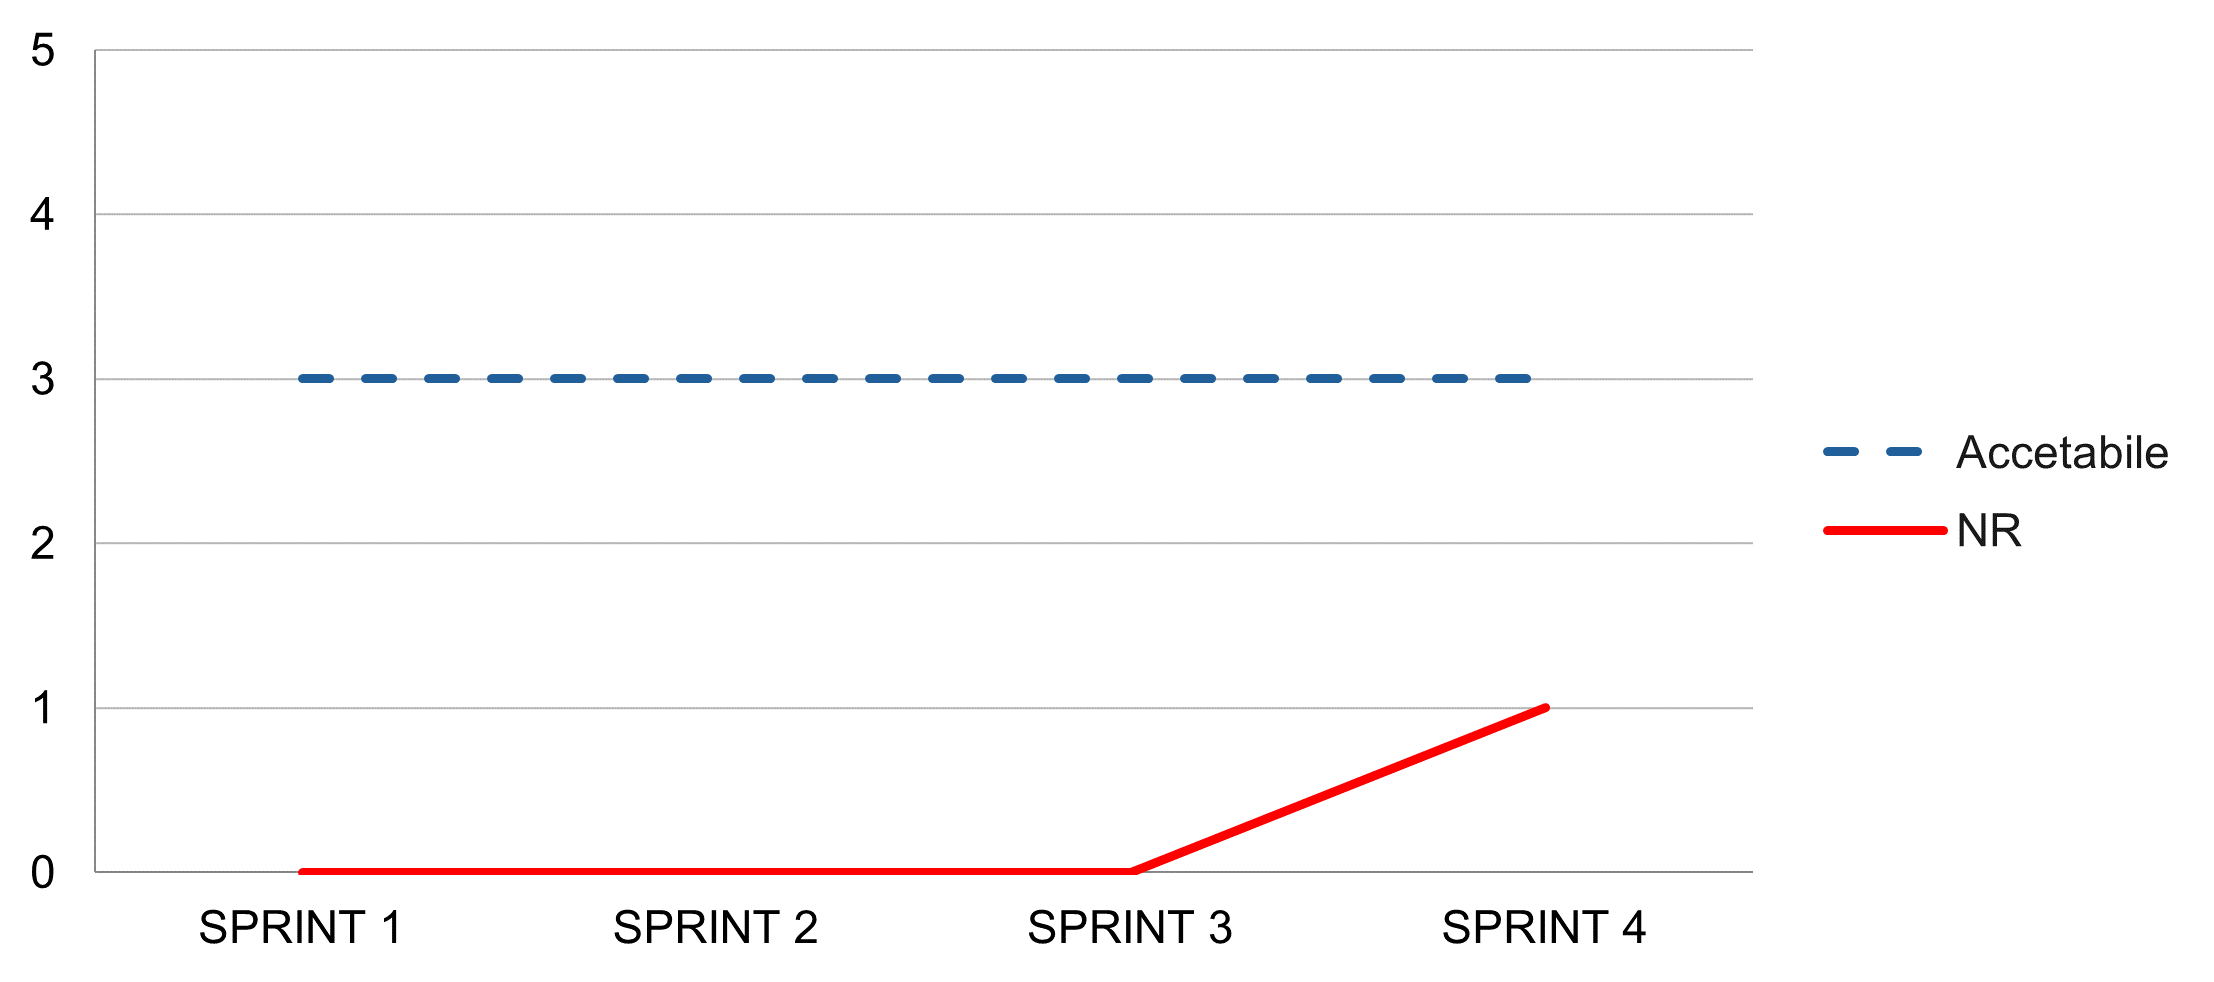
\includegraphics[width=1\textwidth]{images/NR.png}
    \caption{Proiezione grafica dei rischi non calcolati.}
    \label{fig:Proiezione grafica dei rischi non calcolati}
\end{figure}
\textbf{\glossterm{RTB}:} Come mostrato dalla proiezione, il quarto \glossterm{Sprint} è stato soggetto ad un rischio non previsto particolarmente limitante. Su suggerimento della proponente, il team ha affrontato un profondo lavoro di \verb|refactoring| del codice fino a quel momento prodotto, che non solo ha comportato un certo dispendio di risorse destinate ad altre attività ma ha limitato e modificato l'organizzazione che il team aveva precedentemente pianificato per il suddetto periodo. Ciononostante, grazie al lavoro svolto negli \glossterm{Sprint} antecedenti e soprattutto alle accortezze adottate nelle fasi di pianificazione, il refacotring non ha comportato problematiche rispetto al preventivo e alle metriche di fornitura.
\end{document}